% xmodcat1.tex  (16/04/20)

%%%%%%%%%%%%%%%%%%%%%%%%%%%%%%%%%%%%%%%%%%%%%%%%%%%%%%%%%%%%%%
\section{Crossed Modules and Cat$^1$-Groups} \label{sect:xmod}

In this section we describe four equivalent categories:
\begin{itemize}
\item
{\catXMod}, the category of crossed modules and their morphisms;
\item
{\catCat1}, the category of cat$^1$-groups and their morphisms; 
\item
{\catGpGpd}, a category of sets with both a group structure 
and a groupoid structure; and 
\item 
{\cattGp}, a subcategory of {\cattCat}.
\end{itemize}
We also describe functors between these categories which exhibit
the various equivalences.


\subsection{Precrossed and Crossed Modules}

Let $S$ and $R$ be groups acting upon themselves by conjugation:
$$
{s_0}^s = s^{-1}s_0s, \qquad {r_0}^r = r^{-1}r_0r.
$$
A \emph{precrossed module}  \index{precrossed module} 
$\calX = (\delta : S \to R )$ 
consists of a group homomorphism $\delta $, \index{boundary} 
called the \emph{boundary} of $\calX$, 
together with an action 
$\alpha : R \to \Aut(S)$ such that $\delta$  is an $R$-morphism.
So, for all $s \in S$  and  $r \in R$,
\begin{center}
\begin{tabular}{c r c l }
\textbf{X1:} &  $\delta(s^r)$   &  =  &  $(\delta s)^r$~.
\end{tabular}
\end{center}
An alternative terminology is to say that  $(S,\delta)$
is a precrossed $R$-module.
\index{source} \index{range} 
The groups $S,R$ are called the \emph{source} and \emph{range} of $\calX$ 
respectively. 

The precrossed module  $\calX$  is a \emph{crossed module} 
\index{crossed module!of groups} 
if it also satisfies, for all  $s_0,s \in S$,
\begin{center}
\begin{tabular}{c r c l }
\textbf{X2:} &  ${s_0}^{\delta s}$  &  =  &  ${s_0}^s$~. 
\end{tabular}
\end{center}

A \emph{morphism of precrossed modules}  
$\alpha : \calX_1 \to \calX_2$ 
is a pair  $\alpha = (\dda, \da)$, where 
$\dda : S_1 \to S_2$ and $\da : R_1 \to R_2$ are homomorphisms satisfying
$$
\delta_2 \circ \dda = \da \circ \delta_1, \; \;
\dda(s^r) = (\dda  s)^{\da r},
$$
making the following diagram commute:
\begin{equation} \label{eq:prexmod-morph} 
\vcenter{\xymatrix{ 
  S_1 \ar[rr]^{\dda} \ar[dd]_{\delta_1}
     && S_2 \ar[dd]^{\delta_2} \\
     &&  \\
  R_1 \ar[rr]_{\da}
     && R_2
}}
\end{equation} 

When  $\calX_1, \calX_2$  are both crossed modules then  $\alpha$
is a \emph{morphism of crossed modules} 
\index{morphism!of crossed modules} 
without any further condition.
We thus obtain the category
{{\catPreXMod}} of precrossed modules and their morphisms,
and the category {\catXMod} of crossed modules and their morphisms.
Furthermore, {\catXMod} is a full subcategory of {\catPreXMod}.

When $\calX_2 = \calX_1$
and $\dda,\da$ are automorphisms then 
$\alpha$  is an automorphism of $\calX_1$. 
The group of automorphisms is denoted 
by $\Aut(\calX_1).$ 

We have to be careful about a notational problem 
which arises because, although we are using right actions,
we are still writing functions of the left.
Thus the group of automorphisms of $R$ has multiplication
$\beta_1 * \beta_2$  given by
%% \begin{equation} \label{eq:autR}
$$ 
(\beta_1 * \beta_2)r \;=\; \beta_2(\beta_1(r))
\quad \mbox{or, more conveniently,} \quad
\beta_2 \beta_1 r~,
$$ 
%% \end{equation}
where $\beta_1$ is applied \emph{first} to $r$, 
and $\beta_2$ \emph{second}.



%%%%%%%%%%%%%%%%%%%%%%%%%%%%%%%%%%%%%%%%
\subsection{Examples of Crossed Modules} \label{subsec:ex-xmod} 

Standard constructions for crossed modules include the following:

\begin{enumerate}
\item A \emph{conjugation crossed module} $(\inc : S \to R)$ 
      \index{conjugation crossed module} 
      is an inclusion of a normal subgroup  $S \unlhd R$,
      where $R$ acts on $S$ by conjugation. 
      The example takes the alternating subgroup $a_4$ 
      of the symmetric group $s_4$. 
{\small 
\begin{verbatim} 
gap> s4 := Group( (1,2,3,4), (3,4) );;  SetName( s4, "s4" ); 
gap> a4 := Subgroup( s4, [(1,2,3),(2,3,4)] );;  SetName( a4, "a4" ); 
gap> X4 := XModByNormalSubgroup( s4, a4 );; 
gap> Display( X4 );
Crossed module [a4->s4] :- 
: Source group has generators:
  [ (1,2,3), (2,3,4) ]
: Range group s4 has generators:
  [ (1,2,3,4), (3,4) ]
: Boundary homomorphism maps source generators to:
  [ (1,2,3), (2,3,4) ]
: Action homomorphism maps range generators to automorphisms:
  (1,2,3,4) --> { source gens --> [ (2,3,4), (1,3,4) ] }
  (3,4) --> { source gens --> [ (1,2,4), (2,4,3) ] }
  These 2 automorphisms generate the group of automorphisms.
\end{verbatim}}
\item An \emph{automorphism crossed module} $(\inn : R \to S)$ 
      \index{automorphism crossed  module}  
      has as range a subgroup $R$
      of the automorphism group  $\mbox{Aut}(S)$  of  $S$  which
      contains the inner automorphism group  $\mbox{Inn}(S)$  of  $S$.
      The boundary maps $s \in S$  to the inner automorphism of $S$ by $s$. 
      In the example the quaternion group $q_8$ has automorphism group 
      isomorphic to $s_4$.  A permutation representation of degree $6$ 
      for this automorphism group is chosen automatically. 
{\small 
\begin{verbatim}
gap> q8 := Group( (1,2,3,4)(5,8,7,6), (1,5,3,7)(2,6,4,8) );; 
gap> SetName( q8, "q8" ); 
gap> X8 := XModByAutomorphismGroup( q8 );; 
gap> Display( X8 );
Crossed module [q8->PAut(q8)] :- 
: Source group q8 has generators:
  [ (1,2,3,4)(5,8,7,6), (1,5,3,7)(2,6,4,8) ]
: Range group PAut(q8) has generators:
  [ (3,6,5,4), (1,6,3)(2,4,5), (3,5)(4,6), (1,2)(4,6) ]
: Boundary homomorphism maps source generators to:
  [ (3,5)(4,6), (1,2)(4,6) ]
: Action homomorphism maps range generators to automorphisms:
  (3,6,5,4) --> { source gens --> [ (1,2,3,4)(5,8,7,6), (1,8,3,6)(2,5,4,7) ] }
  (1,6,3)(2,4,5) --> { source gens --> 
[ (1,8,3,6)(2,5,4,7), (1,2,3,4)(5,8,7,6) ] }
  (3,5)(4,6) --> { source gens --> [ (1,2,3,4)(5,8,7,6), (1,7,3,5)(2,8,4,6) 
 ] }
  (1,2)(4,6) --> { source gens --> [ (1,4,3,2)(5,6,7,8), (1,5,3,7)(2,6,4,8) 
 ] }
  These 4 automorphisms generate the group of automorphisms.
\end{verbatim}} 
\item A \emph{zero boundary crossed module} $(0 : M \to R)$ 
      \index{$R$-module} 
      has an $R$-module $M$ as source and $\partial = 0$.
\item Any homomorphism  $\partial : S \to R$,  with $S$ abelian
      and $\im\ \partial$ in the centre of $R$, provides a crossed module
      with  $R$  acting trivially on  $S$.
\item A \emph{central extension crossed module} 
      \index{central extension crossed  module} 
      has as boundary a surjection
      $\partial : S \to R$ with central kernel,
      where $r \in R$ acts on $S$ by conjugation with $\partial^{-1}r$.
\item The \emph{direct product} of  
      \index{direct product!of crossed modules} 
      $\calX_1 = (\partial_1 : S_1 \to R_1)$ 
      and  $\calX_2 = (\partial_2 : S_2 \to R_2)$  is
      $ \calX_1 \times \calX_2 = 
        (\partial_1 \times \partial_2 : S_1 \times S_2 \to R_1 \times R_2)$
      with  $R_1, R_2$  acting trivially on  $S_2,\ S_1$  respectively.
\end{enumerate}

\medskip
Here is a verification for the fifth example. 
Suppose $s_1,s_2 \in \partial^{-1}r$. 
Then $s_2 = s_1k$ for some $k \in \ker{\partial}$, 
so $s^{s_2} = s^{s_1k} = s_1^{-1}(k^{-1}sk)s_1 = s^{s_1}$, 
and the action is well-defined. 
The two axioms are then easily verified.

%%%%%%%%%%%%%%%%%%%%%%%%%%%%%%%%%%%%%%%%%%%%%%%%%%%%%%%%%%%%%%%%%%%%%%%%
\subsection{Properties of Crossed Modules} \label{subs:xmod_prop}

\begin{lem}\quad
\begin{enumerate}[{\rm (i)}]
\item~ \index{kernel!of a crossed module} 
The kernel $K$ of  $\partial$  is  central in $S$, and so is abelian.
\item~ \index{cokernel!of a crossed module} 
The image $J = \im\partial$ is normal in $R$,
and so we may define  $C = \coker\partial = R/J$,
with natural map $\nu : R \to C$, 
and hence obtain an exact sequence of groups
$$
1 \quad \longrightarrow \quad 
J \quad \stackrel{\iota}{\longrightarrow} \quad 
R \quad \stackrel{\nu}{\longrightarrow} \quad 
C \quad \longrightarrow \quad 
1~.
$$
\item~
The group  $J$ acts trivially on the centre  $ZS$  of  $S$,
and so trivially on $K$.
Hence  $K$  inherits an action of $C$, making $K$ a $C$-module 
with  $k^{Jr} := k^r$, 
and giving a crossed module $(\nu\partial|_{K} : K \to C)$.
\item~
If  $\partial' : S \to J$ is the restriction of $\partial$,
there is an exact sequence of $R$-groups
$$
1 \quad \longrightarrow \quad 
K \quad \longrightarrow \quad 
S \quad \stackrel{\partial'\,}{\longrightarrow} \quad 
J \quad \longrightarrow \quad 
1~.
$$
\item~
The image  $J$ acts trivially on the abelianisation  
$S^{\ab} = S/[S,S]$  of  $S$, and so  $S^{\ab}$
is also a $C$-module, with action
\begin{equation} \label{eq:Jaction}
([S,S]s)^{(Jr)} \quad = \quad [S,S](s^r)~.
\end{equation}
\end{enumerate}
\end{lem}
\begin{pf}\quad
\begin{enumerate}[(i)]
\item~
If  $k \in K$  and  $s \in S$ then, by \textbf{X2},
$$
s^1 ~=~ s^{\partial k} ~=~ s^k ~=~ k^{-1}sk
\qquad \text{and so} \qquad
ks ~=~ sk\,.
$$
\item~
The conjugate of $\partial s$ by $r \in R$ is 
$r^{-1}(\partial s)r ~=~ (\partial s)^r ~=~ \partial(s^r) \in J$. 
\item~
If  $z \in ZS$ then, by \textbf{X2}, ~$z^{\partial s} = s^{-1}zs = z$. 
Then $\nu(\partial k) = J(\partial k)$ and 
$$
\nu\partial(k^{Jr}) ~=~ J(\partial(k^r)) ~=~ J((\partial k)^r) 
~=~ (Jr^{-1})(J(\partial k))(Jr) ~=~ (\nu\partial k)^{Jr}. 
$$
\item~
The kernel of $\partial'$ is $K$ and $\partial'$ is surjective.
\item~
$$
[S,S]1 \;=\; [S,S][s_1,s_2^{-1}] \;=\; [S,S]\,s_2^{\partial s_1}\,s_2^{-1}
\qquad\Rightarrow\qquad
[S,S]s_2 \;=\; [S,S]s_2^{\partial s_1}~.
$$
Hence $J$ acts trivially on $S^{\ab}$, and it is easy to check that 
(\ref{eq:Jaction}) defines an action.
\end{enumerate}
\end{pf}


%%%%%%%%%%%%%%%%%%%%%%%%%%%%%%%%%%%%%%%%%%%%%%%%%%%%%%%%%%%%%%%%%%%%%%%%%%%%%
\subsection{Sub-crossed modules} \label{subs:subxmods}

\begin{defn} \index{subcrossed module}
A crossed module $\calX_1 = (\partial_1 : S_1 \to R_1)$
is a sub-crossed module of $\calX = (\partial : S \to R)$,
written $\calX_1 \leqslant \calX$, if
\begin{itemize}
\item $S_1,R_1$ are subgroups of $S,R$ respectively,
\item $\partial_1$ is the restriction of $\partial$ to $S_1$,
\item the action of $R_1$ on $S_1$ is induced by the action of $R$ on $S$.
\end{itemize}
\end{defn}

$$
\xymatrix{ 
  S_1 \ar[rr]^{i_{S_1}} \ar[dd]_{\partial_1}
     && S \ar[dd]^{\partial} \\
     &&  \\
  R_1 \ar[rr]_{i_{R_1}}
     && R
}
$$

\begin{defn} \index{inclusion morphism} 
The \emph{inclusion morphism} 
$i = (i_{S_1},i_{R_1}) : \calX_1 \to \calX$
consists of the two subgroup inclusions
$i_{S_1} : S_1 \to S$ and $i_{R_1} : R_1 \to R$.
\end{defn}

\begin{defn} \index{normal crossed module} 
The sub-crossed module $\calX_1$ is a 
\emph{normal sub-crossed module} of $\calX$, 
written $\calX_1 \unlhd \calX$, if
\begin{enumerate}[{\rm (a)}]
\item $R_1 \unlhd R$,
\item ${s_1}^r \in S_1$ for all $r \in R,~ s_1 \in S_1$,
\item $s^{-1}s^{r_1} \in S_1$ for all $r_1 \in R_1,~ s \in S$.
\end{enumerate}
\end{defn}

\noindent
Note that these conditions imply that $S_1 \unlhd S$, 
for ${s_1}^s = {s_1}^{\partial s}$ by {\bf X2:} 
and belongs to $S_1$ by (b).

\begin{prop}
Given two normal sub-crossed modules $\calX_1, \calX_2$ of $\calX$, 
there is a third normal sub-crossed module of $\calX$ 
called the \emph{commutator sub-crossed module} 
$[\calX_1,\calX_2]$, having
\begin{itemize}
\item source group $[S_1,S_2]$,
\item range group $[R_1,R_2]$,
\item the restriction $\partial'$ of $\partial$ to $[S_1,S_2]$ 
as boundary map. 
\end{itemize}
\end{prop}
\begin{pf}
First note that $\partial'[s_1,s_2] = [\partial s_1, \partial s_2]$, 
and that $[s_1,s_2]^{r_1} = [{s_1}^{r_1}, {s_2}^{r_1}]$, 
so $[\calX_1,\calX_2]$ is a sub-crossed module of $\calX$.
To show normality we check that
\begin{enumerate}[{\rm (a)}]
\item ~$[R_1,R_2] \unlhd R$, 
since $r^{-1}[r_1,r_2]r = [r^{-1}r_1r,r^{-1}r_2r]$, 
\item ~$[s_1,s_2]^r = [{s_1}^r,{s_2}^r] \in [S_1,S_2]$,
\item ~The product $s^{-1}s^{[r_1,r_2]}$ may be expanded as  
$$ 
\left[s^{-1}s^{r_1^{-1}}\right]
\left[\left(s^{r_1^{-1}}\right)^{-1}\left(s^{r_1^{-1}}\right)^{r_2^{-1}}\right] 
\left[\left(s^{r_1^{-1}r_2^{-1}}\right)^{-1}
      \left(s^{r_1^{-1}r_2^{-1}}\right)^{r_1}\right] 
\left[\left(s^{r_1^{-1}r_2^{-1}r_1}\right)^{-1}
      \left(s^{r_1^{-1}r_2^{-1}r_1}\right)^{r_2}\right], 
$$
and each of the four pairs of terms has the form $s^{-1}s^{r_0}$, 
and so is in $S_1$. 
\end{enumerate}
\end{pf}



%%%%%%%%%%%%%%%%%%%%%%%%%%%%%%%%%%%%%%%%%%%%%%%%%%%%%%%%%%%%%%%%%%%%%%%%%%%%%
\subsection{Properties of morphisms of crossed modules} 
\label{subs:mor-props}

Let $\mu = (\ddm,\dm) : \calX \to \calX'$  be a morphism of crossed modules.
The kernel of $\mu$ is the sub-crossed module
$$
\ker\mu ~=~ (\partial\mid_{\ker\ddm} \,:\, \ker\ddm \to \ker\dm)
$$
of $\calX$, as shown in the following diagram.
$$
\xy
\xymatrix{
    \ker\ddm \ar[dd]_{\partial\mid_{\ker\ddm}}
               \ar[rr]^i
    &&    S  \ar[rr]^{\ddm} 
             \ar[dd]^{\partial} 
      &&  S' \ar[dd]^{\partial'}  \\
    &&&& \\
    \ker\dm \ar[rr]_i
    &&    R  \ar[rr]_{\dm}
      &&  R' \\ 
}
\endxy
$$
This statement is justified by the following:
$$
s \in \ker\ddm ~\Leftrightarrow~
\ddm s = 1 ~\Leftrightarrow~ 
\partial'\ddm s = 1 ~\Leftrightarrow~ 
\dm\partial s = 1 ~\Leftrightarrow~ 
\partial s \in \ker\dm.
$$

\begin{lem} \index{kernel!of crossed module morphism} 
The kernel of $\mu$ is a normal sub-crossed module of $\calX$.
\end{lem}
\begin{pf}
\begin{enumerate}[(a)]
\item~ $\ker\dm \unlhd R$,
\item~ if $\ddm s_1 = 1$ then 
$\ddm(s_1^r) = (\ddm s_1)^{\dm r} = 1^{\dm r} = 1$, 
so $s_1^r \in \ker\ddm$, 
\item~ if $\dm r_1 = 1$ then 
$\ddm((s^{-1})^{r_1}s) 
 = \left(\ddm s^{-1}\right)^{\dm r_1}\left(\ddm s\right) 
 = 1$,
so $(s^{-1})^{r_1}s \in \ker\ddm$. 
\end{enumerate}
\end{pf}

\begin{thm}
Given a normal sub-crossed module $\calX_1$
of a crossed module $\calX$, there is a quotient crossed module
$$
\calX/\calX_1 ~=~ ( \delta : S/S_1 \to R/R_1 )
$$
where the action is defined by
$$
(S_1s)^{R_1r} ~:=~ S_1(s^r)
$$
and the boundary map is given by
$$
\delta (S_1s) ~:=~ R_1(\partial s).
$$
\end{thm}
\begin{pf}
We first check that we do have an action:
$$
(S_1s)^{R_1r}(S_1s')^{R_1r} ~=~
(S_1(s^r))(S_1({s'}^r)) ~=~
S_1(s^r)({s'}^r) ~=~
S_1(ss')^r ~=~
(S_1(ss'))^{R_1r},
$$
$$
((S_1s)^{R_1q})^{R_1r} ~=~
(S_1(s^q))^{R_1r} ~=~
S_1(s^q)^r ~=~
S_1(s^{qr}) ~=~
(S_1s)^{R_1(qr)}.
$$
Then we check the crossed module axioms:
$$
\textbf{M1:}\quad
\delta((S_1s)^{R_1r}) \,=\,
\delta(S_1 s^r) \,=\,
R_1 \partial(s^r) \,=\,
R_1 r^{-1}(\partial s)r \,=\,
(R_1r^{-1})(R_1 \partial s)(R_1r) \,=\,
(\delta(S_1s))^{R_1r},
$$
$$
\textbf{M2:}\quad
(S_1s')^{\delta(S_1s)} ~=~
(S_1s')^{R_1(\partial s)} ~=~
S_1 (s')^{\partial s} ~=~
S_1 s^{-1}s's ~=~
(S_1 s^{-1})(S_1 s')(S_1 s).\qquad\qquad\qquad
$$
\end{pf}

\begin{thm} \label{thm:tp-top}
[from Tim Porter's Topology paper \cite{porter:top}]
\mbox{}\\
Every crossed module is a quotient of normal inclusion crossed modules.
\end{thm}
\begin{pf}
Given  $\calX = (\partial : S \to R)$,
consider the diagram 
\begin{equation} \label{eq:tp-quotient}
\vcenter{\xy
\xymatrix{
    1 \ar[dd]_{0}  \ar[rr]^{0}
    &&    S  \ar[rr]^{1} 
             \ar[dd]^{\epsilon} 
      &&  S  \ar[dd]^{\partial}  \\
    &&&& \\
    S \ar[rr]_{\zeta}
    &&    R \ltimes S  \ar[rr]_{h}
      &&  R \\
    \Gamma_1\calX && \Gamma_0\calX && \calX \\ 
}
\endxy} 
\end{equation}

\bigskip
where the crossed modules  $\Gamma_0\calX$ and $\Gamma_1\calX$  are given by
\begin{itemize}
\item~ 
$\epsilon s = (1,s), \quad 
\zeta s = (\partial s, s^{-1}), \quad
{s_1}^{(r,s)} = s^{-1} {s_1}^r s = {s_1}^{r(\partial s)}$,
\item~ 
$h(r,s) = r(\partial s), \quad
(r_1,s)^r = (r^{-1}r_1r, s^r)$.
\end{itemize}

\noindent 
The proof requires four verifications. 
Recall that in the semidirect product $R \ltimes S$ we have 
\begin{equation} \label{eq:sdp-rules}
(r,s)(r',s') = (rr',s^{r'}s') \qquad \mathrm{and} \qquad 
(r,s)^{-1} = (r^{-1},(s^{-1})^{r^{-1}}). 
\end{equation}

\bigskip\noindent {\bf (a)}~ 
Verification that $(\epsilon : S \to R \ltimes S)$ is a crossed module.

\bigskip\noindent{\bf X1:}\quad
$(\epsilon s_1)^{(r,s)} ~=~  
(r^{-1},(s^{-1})^{r^{-1}})(1,s_1)(r,s) ~=~ 
(1,s^{-1}s_1^rs) ~=~ 
\left(1,s_1^{(r,s)}\right) ~=~
\epsilon\left(s_1^{(r,s)}\right).$

\bigskip\noindent{\bf X2:}\quad
${s_1}^{\epsilon s} ~=~ {s_1}^{(1,s)} ~=~ s^{-1}s_1s.$

\bigskip\noindent {\bf (b)}~ 
Verification that $(1,h)$ and $(\epsilon,\delta)$ 
are morphisms of crossed modules.

\bigskip
(i)~ $h \epsilon s ~=~ h(1,s) ~=~ \partial s$,

\bigskip
(ii)~ 
$\left\{ 
\begin{array}{rcl}
1({s_1}^{(r,s)}) & = & 
{s_1}^{(r,s)} ~=~ s^{-1}{s_1}^rs, \\
(1s_1)^{h(r,s)} & = &
{s_1}^{r(\partial s)} ~=~ 
s^{-1}{s_1}^rs. \\
\end{array}\right.$

\bigskip
(ii$^{\prime}$)~ 
$\left\{ 
\begin{array}{rcl}
\epsilon({s_1}^s) & = & 
(1,{s_1}^s) ~=~ (1,s^{-1}s_1s), \\
(\epsilon s_1)^{\partial s} & = &
(1,s_1)^{\partial s} ~=~ 
(1,s_1)^{(1, \partial s)} ~=~ (1,{s_1}^{\partial s})~=~
(1, s^{-1}s_1s). \\
\end{array}\right.$

\bigskip\noindent {\bf (c)}~ 
Verification that $(0,\zeta)$ is the inclusion of a normal sub-crossed module.

\bigskip\noindent
We only need to show that ${s_1}^{-1} {s_1}^{\zeta s} = 1$.
$$
{s_1}^{-1} {s_1}^{\zeta s} ~=~
{s_1}^{-1} {s_1}^{(\partial s, s^{-1})} ~=~
{s_1}^{-1} s {s_1}^{\partial s} s^{-1} ~=~ 1.
$$

\bigskip\noindent {\bf (d)}~ 
Verification that $h\zeta = 0$.
$$
h \zeta s ~=~ h(\partial s, s^{-1}) ~=~ (\partial s)(\partial s^{-1}) ~=~ 1.
$$
\end{pf}

\begin{cor}
In the previous result $\Gamma_0, \Gamma_1 : {\XMod} \to {\XMod}$ are functors
and $(0,\zeta) : \Gamma_1 \to \Gamma_0$ is a natural transformation.
\end{cor}

Note that, in diagram (\ref{eq:tp-quotient}),  
$(h : R \ltimes S \to R)$ is \emph{not} in general a crossed module,
so the right-hand square is not a crossed square 
(see Chapter \ref{sect:xsq-cat2}).

\bigskip
We may extend the above Theorem to morphisms of crossed modules. 
In the diagram (\ref{eq:tp-quotient-morphism}) below, 
$(\sigma,\rho) : \calX_1 
 = (\partial : S \to R) \to \calX_2 = (\delta : Q \to P)$ 
is a morphism of crossed modules, 
and both of these crossed modules are expressed as quotients of 
normal inclusion crossed modules. 
There are morphisms 
$(\sigma,\gamma) : \Gamma_0\calX_1 = (\epsilon : S \to R \ltimes S) 
 \to \Gamma_0\calX_2 = (\eta : Q \to P \ltimes Q)$ 
and $(1,\sigma) : \Gamma_1\calX_1 \to \Gamma_1\calX_2$ 
where $\gamma(r,s) = (\rho r, \sigma s)$ and 
$\eta\sigma s = (1,\sigma s) = \gamma(1,s) = \gamma\epsilon s$. 

\begin{equation} \label{eq:tp-quotient-morphism}
\vcenter{\xy
\xymatrix{
     & 1 \ar[dd]^{0} \ar[rr]^0
         &   & Q \ar[rr]^{1} \ar[dd]^{\eta} 
                 &   & Q \ar[dd]^{\delta}  \\
     &   &   &   &   & \\ 
     & Q \ar[rr]^(0.35){\theta} 
         &   & P \ltimes Q \ar[rr]^{k} 
                 &   & P  \\ 
  1 \ar[dd]_{0} \ar[rr]^(0.6){0} \ar[ruuu]^(0.6){1} 
     &   & S \ar[rr]^(0.6){1} \ar[dd]_{\epsilon} \ar[ruuu]^(0.6){\sigma}  
             &   & S \ar[dd]_{\partial} \ar[ruuu]^(0.6){\sigma} 
                     & \\
     &   &   &   &   & \\
  S \ar[rr]_(0.4){\zeta} \ar[ruuu]_(0.4){\sigma} 
     &   & R \ltimes S \ar[rr]_{h} \ar[ruuu]_(0.4){\gamma} 
             &   & R \ar[ruuu]_(0.4){\rho} 
                     & \\
}
\endxy} 
\end{equation}


\bigskip
%%%%%%%%%%%%%%%%%%%%%%%%%%%%%%%%%%%%%%%%%%%%%%%%%%%%%%%%%%%%%%%%%%%%%%%%%%%%%
\subsection{Peiffer subgroup of a precrossed module} \label{subs:Peiffer}

We shall construct from any precrossed module $\calQ = (\delta : Q \to R)$ 
a crossed module $\calX = (\partial : Q/P \to R)$ whose source is a suitable 
quotient of $Q$. 

Given  $\calQ = (\delta : Q \to R)$
the \emph{Peiffer commutators}  of  $\calQ$  are elements of the form
\index{Peiffer commutator} \index{commutator!Peiffer}
$$
\langle q_1,q_2 \rangle 
\quad=\quad 
%%% q_1^{-1}\,q_2^{-1}\,q_1\,{q_2}^{\delta q_1},
(q_2^{-1})^{q_1}\,{q_2}^{\delta q_1},
\qquad \mbox{where} \quad q_1,q_2 \in Q,
$$
so that
$$
\langle q_1,q_2 \rangle \,=\, 1 \quad \Leftrightarrow \quad
{q_2}^{\delta q_1} \;=\; q_1^{-1}\,q_2\,q_1
$$
The subgroup  $P$  of  $Q$  generated by the Peiffer commutators 
is known as the \emph{Peiffer subgroup} of  $\calQ$.

\begin{lem} \label{lem:Peiffer} \index{Peiffer subgroup} 
\quad\\
\vspace{-5mm}
\begin{enumerate}[{\rm (a)}]
\item~ 
$\langle q_1,1 \rangle \;=\; 1 \;=\; \langle 1,q_2 \rangle$~; 
\item~
$\delta \langle q_1,q_2 \rangle \;=\; 1_R$~;
\item~
$\langle q_1q_3,q_2 \rangle 
\;=\; \langle q_1,q_2 \rangle^{q_3}\;\langle q_3,{q_2}^{\delta q_1} \rangle $~;
\item~
$\langle q_1,q_2q_3 \rangle 
\;=\; \langle q_1,q_3 \rangle\;\langle q_1,q_2\rangle^{{q_3}^{\delta q_1}} $~;
\item~
$\langle q_1, q_2 \rangle^r
\;=\;
\langle {q_1}^r,{q_2}^r \rangle$~; 
\item~ 
$\langle q_1,q_2 \rangle^{-1} 
\;=\; \langle q_1^{-1}, q_2^{\delta q_1} \rangle^{q_1}$~. 
\end{enumerate}
\end{lem}
\begin{pf}
Part (a) is immediate, and part (b) follows from  
$\delta({q_2}^{\delta q_1}) \;=\; 
(\delta q_1)^{-1}(\delta q_2)(\delta q_1)$.
The remaining parts follow on expanding the Peiffer elements,
and are closely related to identities for commutators and
crossed pairings (see Subsection \ref{subs:xp}):
\begin{eqnarray*}
~\langle q_1q_3,q_2 \rangle  
& = & 
\left[ q_3^{-1}q_1^{-1}q_2^{-1}q_1{q_2}^{\delta q_1} q_3 \right] 
\left[ q_3^{-1} ({q_2}^{\delta q_1})^{-1} q_3 {q_2}^{\delta(q_1q_3)} \right] 
~=~
\langle q_1,q_2 \rangle ^{q_3}\;\langle q_3, {q_2}^{\delta q_1} \rangle \;, 
\\
~\langle q_1,q_2q_3 \rangle  
& = &
\left[ q_1^{-1}q_3^{-1}q_1 {q_3}^{\delta q_1} \right]  
\left[ ({q_3}^{\delta q_1})^{-1} q_1^{-1}q_2^{-1} q_1 (q_2 q_3)^{\delta q_1} \right] 
~=~
\langle q_1,q_3 \rangle \;
\langle q_1,q_2 \rangle ^{{q_3}^{\delta q_1}} \;, 
\\
\langle {q_1}^r,{q_2}^r \rangle 
& = & 
(q_1^{-1})^r (q_2^{-1})^r {q_1}^r ({q_2}^r)^{(r^{-1}(\delta q_1)r)} 
~=~ 
(q_1^{-1} q_2^{-1} q_1 {q_2}^{\delta q_1})^r \;, 
\\ 
~\langle q_1,q_2 \rangle^{-1} 
& = & 
\left(q_2^{\delta q_1}\right)^{-1}q_1^{-1}q_2q_1 
~=~ q_1^{-1}\left[q_1 \left(q_2^{\delta q_1}\right)^{-1}
      q_1^{-1}\left(q_2^{\delta q_1}\right)^{\delta q_1^{-1}}\right]q_1 
~=~ \langle q_1^{-1}, q_2^{\delta q_1} \rangle^{q_1} \;. 
\end{eqnarray*} 
\end{pf}

\bigskip 
The following result follows immediately from these identities.

\begin{cor}
Let  $\calQ = (\delta : Q \to R)$  be a precrossed module.
Then the set  $P$  of Peiffer commutators in $\calQ$
is a subgroup of  $\ker \delta$;
is normal in  $Q$;  and is  $R$-invariant.
\end{cor}

\begin{prop}
If  $(\dda,\da) : \calQ_1 \to \calQ_2$  is a morphism of precrossed modules,
then Peiffer commutators in $Q_1$  are mapped to Peiffer commutators
in $Q_2$.
\end{prop}
\begin{pf}
The source map  $\dda$  is compatible with the Peiffer pairing:
\begin{eqnarray*}
\dda \langle q_1, q_2 \rangle & = &
(\dda q_1)^{-1}\,(\dda q_2)^{-1}\,(\dda q_1)\,(\dda({q_2}^{\delta_1q_1})) \\
 & = &
(\dda q_1)^{-1}\,(\dda q_2)^{-1}\,(\dda q_1)\,(\dda q_2)^{\da\delta_1q_1} \\
 & = &
(\dda q_1)^{-1}\,(\dda q_2)^{-1}\,(\dda q_1)\,(\dda q_2)^{\delta_2(\dda q_1)}\\
 & = &
\langle\,\dda q_1,\,\dda q_2\,\rangle~.
\end{eqnarray*}
\end{pf}

\begin{prop}
Let   $\calQ = (\delta : Q \to R)$  be a precrossed module.
Then there is a crossed module  $\calX = (\partial : S \to R)$
and a morphism of precrossed modules  $(\nat,1) : \calQ \to \calX$
such that  $(\nat,1)$  is universal for morphisms from  $\calQ$
to crossed modules over $R$.
\end{prop}
\begin{pf}
Let  $P$  be the Peiffer group of  $\calQ$.
Then the quotient group  $S = Q/P$  is well-defined,
$\nat : Q \to S$  is the natural quotient map,
and  $S$  inherits an  $R$-action and an $R$-morphism: 
$$
(Pq)^r = P(q^r)~,
\qquad \qquad
\partial : S \to R,\; (Pq) \mapsto \delta q~.
$$
So  $\calX = (\partial : S \to R)$  is a precrossed module.
By definition of  $P$, we have  $s_1^{-1}s_2s_1 = {s_2}^{\partial s_1}$
for all  $s_1,s_2 \in S$,  and so  $\calX$  is a crossed module.
The quotient morphism  $(\nat,1)$  is clearly a morphism of 
precrossed modules.

$$
\xy
\xymatrix{
   &&&&&&  \\
   &      S' \ar[dd]_{\partial'}
    &&    Q  \ar[rr]^(0.4){\nat} 
             \ar[ll]_{n'}  
             \ar[dd]^{\delta} 
      &&  S = Q/P  \ar[dd] ^{\partial}  
           \ar `u[-1,-1] `[0,-4]_{\theta} [0,-4]
        &    \\
   &&&&&& \\
   &      R 
    &&    R  \ar[ll]^1
             \ar[rr]_1
      &&  R
        & \\ 
}
\endxy
$$

\bigskip
If  $\calX' = (\partial' : S' \to R)$  is a crossed module
and if  $(n',1) : \calQ \to \calX'$  is a precrossed module morphism,
then there is a unique crossed module morphism  
$(\theta,1) : \calX \to \calX'$
such that  $(\theta,1)\circ(\nat,1) = (n',1)$  where  $\theta(Pq) = n'q$.
\end{pf}

\begin{example}
In the following \GAP~ run the Peiffer subgroup is cyclic of order $4$. 
{\small 
\begin{verbatim}
gap> b1 := (11,12,13,14,15,16,17,18);;  b2 := (12,18)(13,17)(14,16);;
gap> d16 := Group( b1, b2 );;
gap> sk4 := Subgroup( d16, [ b1^4, b2 ] );;
gap> SetName( d16, "d16" );  SetName( sk4, "sk4" );
gap> bdy16 := GroupHomomorphismByImages( d16, sk4, [b1,b2], [b1^4*b2,b2] );;
gap> aut1 := GroupHomomorphismByImages( d16, d16, [b1,b2], [b1^5,b2] );;
gap> aut2 := GroupHomomorphismByImages( d16, d16, [b1,b2], [b1,b1^4*b2] );;
gap> aut16 := Group( [ aut1, aut2 ] );;
gap> act16 := GroupHomomorphismByImages( sk4, aut16, [b1^4,b2], [aut1,aut2] );;
gap> P16 := PreXModByBoundaryAndAction( bdy16, act16 );
gap> P := PeifferSubgroup( P16 );
Group([ (11,15)(12,16)(13,17)(14,18), (11,13,15,17)(12,14,16,18) ])
gap> X16 := XModByPeifferQuotient( P16 );;
Peiffer([d16->sk4])
gap> Display( X16 );
Crossed module Peiffer([d16->sk4]) :- 
: Source group has generators:
  [ f1, f2 ]
: Range group has generators:
  [ (11,15)(12,16)(13,17)(14,18), (12,18)(13,17)(14,16) ]
: Boundary homomorphism maps source generators to:
  [ (12,18)(13,17)(14,16), (11,15)(12,14)(16,18) ]
  The automorphism group is trivial
\end{verbatim}} 
\end{example} 

\vspace*{5mm}
The following result, 
which gives a normal generating set for the Peiffer group, 
is Proposition 3 of \cite{brow:hueb}.
The method of proof was suggested by Philip Higgins.

\begin{prop}
Given the following ingredients:
\begin{itemize}
\item
$\calQ \;=\; (\delta : Q \to R)$, a precrossed module;
\item
$\Gamma$, a generating set for $Q$, closed under the action of $R$;
\item
$P$, the Peiffer group of $\calQ$;
\item
$E$, the set of Peiffer elements  
$\{\langle a,b \rangle \;\mid\; a,b \in \Gamma\}$~;
\end{itemize}
then  $P$  is the normal closure of $E$ in $\Gamma$.
\end{prop}
\begin{pf}
Let  $P'$  be the normal closure of  $E$  in  $Q$,  so that
$$
P' \;\normeq\; P \;\normeq\; \ker\delta \;\normeq\; Q~.
$$
If  $P \neq P'$  then there is some
$z = \langle x,y \rangle \in P \setminus P'$
such that
$P'z \neq P'$  in  $Q/P'$~.
Since
$$
P'z \neq P' \quad\Rightarrow\quad
zP' \neq P' \quad\Rightarrow\quad
y^{\delta x}\,P' \neq (x^{-1}yx)P' \quad\Rightarrow\quad
P'y^{\delta x} \neq P'(x^{-1}yx)~,
$$
we need to show that
$P'\,y^{\delta x} \;=\; P'(x^{-1}yx)$  
for all $\langle x,y \rangle \in P'$~.

Since  $\Gamma$  is  $R$-invariant,
part (d) of Lemma \ref{lem:Peiffer} shows that  $E$  is  $R$-invariant,
and hence  $P'$  is  $R$-invariant.
Since  $P' \normeq Q$,
form  $S' = Q/P'$  with $R$-action  $(P'q)^r = P'(q^r)\,$.
The homomorphism  $\delta$  induces
$\partial' : S' \to P',\; P'q \mapsto \delta q$,  and
$\calX' = (\partial' : S' \to R)$  is a precrossed module since
$$
\partial'((P'q)^r) \;=\;
\partial'(P'(q^r)) \;=\;
\delta q^r \;=\;
r^{-1}(\delta q)r \;=\;
r^{-1}(\partial'(P'q))r~.
$$

Since  $\Gamma$  generates  $Q$  as a group,  the set of cosets
$C' = \{P'a \,\mid\, a \in \Gamma\}$
generates  $S'$ and, for all  $P'a,P'b \in C'$~,
\begin{equation}\label{eq:X2eqn}
(P'a)^{\partial'(P'b)} \;=\;
(P'a)^{\delta b} \;=\;
P'(a^{\delta b}) \;=\;
P'(b^{-1}ab) \;=\;
(P'b)^{-1}(P'a)(P'b)~.
\end{equation}

For fixed  $b$,  the set of  $P'a$  satisfying (\ref{eq:X2eqn})
is a subgroup of  $S'$~:
$$
((P'a)(P'c))^{\partial'(P'b)} \;=\;
(P'a)^{\partial'(P'b)}(P'c)^{\partial'(P'b)} \;=\;
(P'b)^{-1}(P'a)(P'c)(P'b)~.
$$
So (\ref{eq:X2eqn}) is true for all  $(P'a) \in S'$  and all  $(P'b) \in C'$~.

Also, the set of  $(P'b) \in C'$  satisfying  (\ref{eq:X2eqn})
is closed under multiplication and inversion since
\begin{itemize}
\item
$(P'a)^{\partial'(P'(bc))} \;=\;
((P'a)^{\delta(b)})^{\delta c} \;=\;
(P'(bc))^{-1}\,(P'a)\,(P'(bc))$~;
\item
$(P'a)^{\partial'(P'b)^{-1}} = P'c \quad\Rightarrow\quad
P'a=(P'b)^{-1}(P'c)(P'b) \quad\Rightarrow\quad
(P'b))(P'a)(P'b)^{-1} = P'c$~.
\end{itemize}
Thus (\ref{eq:X2eqn}) holds for \emph{all}  $P'a, P'b \in C'$~.
\end{pf}



%%%%%%%%%%%%%%%%%%%%%%%%%%%%%%%%%%%%%%%%%%%%%%%%%%%%%%%%
\subsection{Free Crossed Modules} \label{subs:free-xmod}
\index{free crossed module}

We first recall a property of free groups which we wish to generalise.
Let  $\Omega$  be a set.
The \emph{free group on $\Omega$} is a group $F$ and a function
$\nu : \Omega \to F$  such that if $G$ is a group and  
$\nu' : \Omega \to G$ a function, then there exists a unique
group homomorphism  $\theta : F \to G$  such that  
$\theta\circ\nu = \nu'$.

$$\xy
\xymatrix{
   &&&&&&  \\
   &      G  
    &&    \Omega  \ar[rr]_{\nu} 
             \ar[ll]^{\nu'}   
      &&  F  \ar `u[-1,-1] `[0,-4]_{\theta} [0,-4]
        &    \\
}
\endxy$$

\bigskip
To construct a particular model for $F = F(\Omega)$ we take an alphabet
consisting of all the elements of $\Omega$ together with their
formal inverses, and take for $F$ the set of all reduced words
in this alphabet with concatenation as the group product
and the empty word as the identity.  The details of this construction
should be familiar to the reader.

We now define a \emph{free precrossed module} in an analogous manner.
The ingredients for the construction are
\begin{itemize}
\item~ a set $\Omega$,
\item~ a group $R$,
\item~ a function $\omega : \Omega \to R$.
\end{itemize}
The resulting construction consists of
\begin{itemize}
\item~ a precrossed module $\calQ = (\delta : Q \to R)$,
\item~ a function  $\nu : \Omega \to Q$  such that  
$\delta\circ\nu = \omega$.
\end{itemize}
The universal property required of this construction 
is that if  $\calQ' = (\delta' : Q' \to R)$
is another precrossed module, and if  $\nu' : \Omega \to Q'$
satisfies  $\delta'\circ\nu' = \omega$,
then there exists a unique morphism of precrossed modules
$(\theta,1) : \calQ \to \calQ'$  such that  
$(\theta,1)\circ(\nu,1) = (\nu',1)$.
$$
\xy
\xymatrix{
   &&&&&&  \\
   &      Q' \ar[ddrr]_{\delta'}
    &&    \Omega  \ar[rr]^{\nu} 
             \ar[ll]_{\nu'}  
             \ar[dd]^{\omega} 
      &&  Q  \ar[ddll] ^{\delta}  
           \ar `u[-1,-1] `[0,-4]_{\theta} [0,-4]
        &    \\
   &&&&&& \\
   &&&    R
      &&& \\ 
}
\endxy$$

\bigskip\noindent
A particular model is obtained as follows:
\begin{itemize}
\item~ the source group $Q$ is the free group $F(\Omega \times R)$,
\item~ the boundary map is defined on generators by 
$\delta(\rho,r) = (\omega\rho)^r = r^{-1}(\omega\rho)r$,
\item~ the action is given by $(\rho,r)^{r'} = (\rho,rr')$,
\item~ the function is given by $\nu(\rho) = (\rho,1)$.
\end{itemize}

\noindent
We observe that
$$
\delta\circ\nu(\rho) ~=~ \delta(\rho,1) ~=~ \omega\rho
\quad\text{for all}\quad  \rho \in \Omega,
$$
and verify {\bf X1:} as follows:
$$
\delta((\rho,r)^{r'}) ~=~
\delta(\rho,rr') ~=~
{r'}^{-1}(r^{-1}(\omega\rho)r)r' ~=~
{r'}^{-1}\,\delta(\rho,r)\,r'~.
$$

To check the universal property we need to define
$\theta : Q \to Q'$  in such a way that  $\theta(\rho,1) = \nu'\rho$.
Since $\theta$ is to preserve the $R$-action, we are forced to define
$$
\theta(\rho,r) ~=~ 
\theta((\rho,1)^r) ~=~
(\nu'\rho)^r 
%~=~ r^{-1}(\nu'\rho)r
~.
$$
This defines $\theta$ on the whole of $Q$, and we verify that $(\theta,1)$
is a morphism of precrossed modules:
\begin{itemize}
\item\quad
$
\delta'\theta(\rho,r) ~=~
\delta'((\nu'\rho)^r) ~=~
r^{-1}(\delta'\nu'\rho)r ~=~
r^{-1}(\omega\rho)r ~=~
\delta(\rho,r) ~,
$
\item\quad
$
\theta((\rho,r)^{r'}) ~=~
\theta(\rho,rr') ~=~
(\nu' \rho)^{rr'} ~=~
(\theta(\rho,r))^{r'} ~.
$
\end{itemize}

We are now in a position to construct the free crossed module
associated to a free precrossed module, simply by factoring out
the Peiffer commutators in  $Q = F(\Omega \times R)$\,:
\begin{eqnarray*}
\langle (\rho_1, r_1), (\rho_2, r_2) \rangle 
& = &
(\rho_1, r_1)^{-1}\,(\rho_2, r_2)^{-1}\,
  (\rho_1, r_1)\,(\rho_2, r_2)^{\delta(\rho_1, r_1)}  \\
& = &
(\rho_1, r_1)^{-1}\,(\rho_2, r_2)^{-1}\,
  (\rho_1, r_1)\,(\rho_2, r_2)^{r_1^{-1}(\omega\rho_1)r_1} \\
& = &
(\rho_1, r_1)^{-1}\,(\rho_2, r_2)^{-1}\,
  (\rho_1, r_1)\,(\rho_2, r_2r_1^{-1}(\omega\rho_1)r_1)~. 
\end{eqnarray*}
We thus obtain a crossed module with source  $C(\omega) = Q/P$\,:
\begin{eqnarray*}
\calF_{\rho} & = & (\partial : C(\omega) \to R)\,, \\
\partial(P(\rho,r)) & = & \delta(\rho,r) ~=~ r^{-1}(\omega\rho)r\,, \\
(P(\rho,r))^{r'} & = & P(\rho,rr')\,.
\end{eqnarray*}

It is often convenient to use an alternative notation for elements in $Q$.
Since  $(\rho,r) = (\rho,1)^r$
we may drop the ``$,1$'' and write  $(\rho)^r$  for  $(\rho,r)$,
and the inverse element by  $(\rho^{-1})^r$\,:
$$
\{(\rho)^r\}^{-1} ~=~
(\rho,r)^{-1} ~=~
\{(\rho,1)^r\}^{-1} ~=~
\{(\rho,1)^{-1})^r ~=~
(\rho^{-1})^r\;.
$$
The action is then given by  
$$
((\rho^{\epsilon})^r)^{r'} ~=~ (\rho^{\epsilon})^{(rr')}
\quad\text{where}\quad \epsilon = \pm 1~.
$$
The Peiffer commutators on generators in this notation are
$$
\langle\,({\rho_1}^{\epsilon_1})^{r_1},\,({\rho_2}^{\epsilon_2})^{r_2}
\,\rangle
~=~
({\rho_1}^{-\epsilon_1})^{r_1}\,({\rho_2}^{-\epsilon_2})^{r_2}\,
({\rho_1}^{\epsilon_1})^{r_1}\,
({\rho_2}^{\epsilon_2})^{r_2 r_1^{-1} (\omega\rho_1) r_1}~.
$$

\bigskip
%%%%%%%%%%%%%%%%%%%%%%%%%%%%%%%%%%%%%%%%%%%%%%%%%%%%%%%
\subsection{The monoid version of free crossed modules}

Given  $Y = \Omega \times R$, define
$$
\bar{Y} ~=~ \{ y^+ : y \in Y \} \;\sqcup\; \{ y^- : y \in Y \}\,.
$$
It is convenient to use an alternative notation, as above:
$$
(\rho^+)^r \;:=\; (\rho,r)^+\,, \quad\quad
(\rho^-)^r \;:=\; (\rho,r)^-\,.
$$
Then  $H = \bar{Y}^{\ast}$ is the free monoid on $\bar{Y}$
with empty word $\lambda$ and elements
$$
(\rho_1^{\epsilon_1})^{r_1}\, (\rho_2^{\epsilon_2})^{r_2}\, 
\cdots (\rho_n^{\epsilon_n})^{r_n}\,, \quad
\rho_i \in \Omega,\; \epsilon_i \in \{+,-\},\; r_i \in R\,. 
$$
The boundary map is the monoid morphism
$$
\bard \;:\; \bar{Y}^{\ast} \to R,\quad
(\rho^+)^r \mapsto r^{-1}(\omega \rho)r,\quad
(\rho^-)^r \mapsto r^{-1}(\omega \rho)^{-1}r.
$$
Then $F(\omega)$ is the quotient monoid  $\bar{Y}^{\ast}/\equiv$
where $\equiv$ is the congruence generated by 
\begin{itemize}
\item~
inverse pairs~ $(y^{\epsilon}y^{-\epsilon},\lambda)$,
\item~
Peiffer pairs~ $(y^{-\epsilon} z^{\eta} y^{\epsilon},
(z^{\eta})^{\bard y^{\epsilon}}), 
\quad \epsilon,\eta \in \{+,-\}, 
\quad -(-) = +,$ \quad etc.
\end{itemize}

In the special case of a group presentation
$$
\calP ~=~ \grp( X, \omega : \Omega \to F(X)),
$$
$\omega\rho$ is a relator and so a word in $F(X)$.
Then  $Y = \Omega \times F(X)$  and  
$H = \bar{Y}^{\ast}$  has elements of the form
$$
(\rho_1^{\epsilon_1})^{u_1}\, (\rho_2^{\epsilon_2})^{u_2}\, 
\cdots (\rho_n^{\epsilon_n})^{u_n}\,, 
$$
and $\ker\partial = \Pi_2(\calP)$ is the $\mathbb{Z}G$-module
of identities among the relators of $\calP$.

\bigskip
\begin{example}
\emph{Consider the following presentation for the quaternion group 
of size $8$.}
$$
X = \{a,b\}, \quad
\Omega = \{\rho_1,\rho_2,\rho_3,\rho_4\}, \quad
\omega : \rho_1 \mapsto a^4,\; \rho_2 \mapsto b^4,\; 
\rho_3 \mapsto abab^{-1},\; \rho_4 \mapsto a^2b^2.\; 
$$
\emph{The identity}
$$
\iota ~=~ (\rho_4^-)\ (\rho_1^+)^{a^2}\ (\rho_4^-)^{a^2}\ (\rho_2^+)
$$
\emph{maps by $\partial$ to}
$$
(b^{-2}a^{-2}).a^{-2}(a^4)a^2.a^{-2}(b^{-2}a^{-2})a^2.(b^4) ~=~ \lambda\,.
$$
\end{example}

\bigskip
\begin{center}
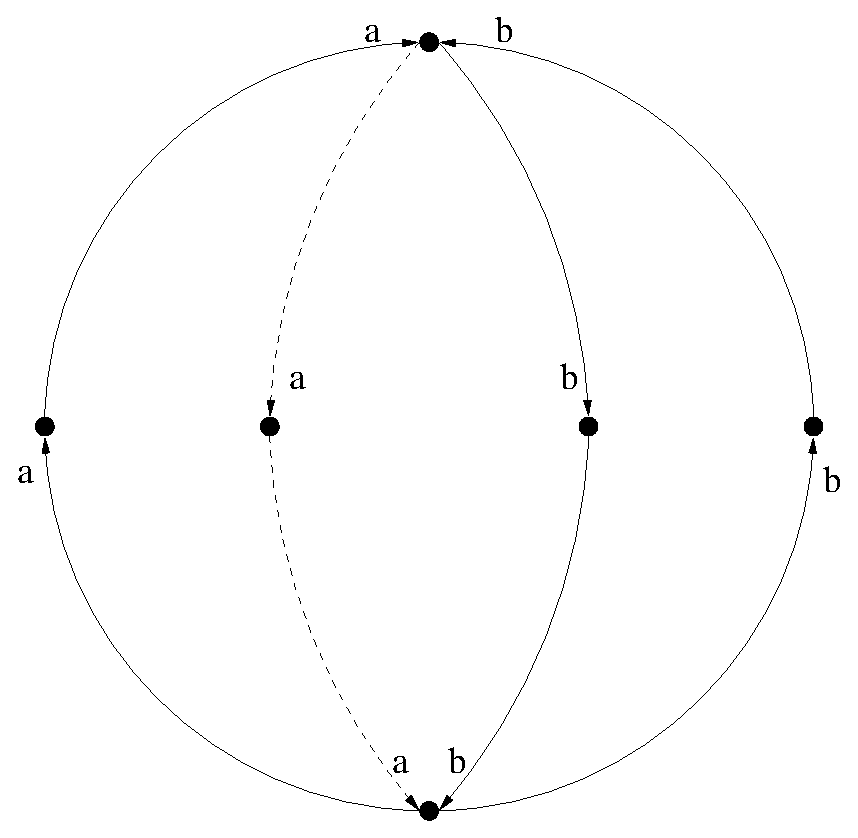
\includegraphics[scale = 0.5]{xmodcat1/q8-vankampen.eps}
%% \input{q8-vankampen.pstex_t} 
\end{center}

In the van Kampen diagram, relators $\rho_1, \rho_2$ and $\rho_4$ (twice) 
tile a sphere as shown above. 
Tracing out $\partial \iota$ we walk around the boundaries of these four tiles, 
in the order back-right; back-left; front-left; front-right;
in such a way that every edge cancels out with its inverse. 


\bigskip 
%%%%%%%%%%%%%%%%%%%%%%%%%%%%%%%%%%%%%%%%%%%%%%%%%%%%%%%%%%%%%%%%%%%%%%%%
\subsection{A Geometric Example of a Crossed Module} \label{subs:geom-ex}

The major geometric example of a crossed module can be expressed
in two ways.
Let $(X,A,a)$ be a based pair of spaces, with  $a \in A \subseteq X$. 
Let  $I=[0,1]$  be the unit interval, $I^2$ the unit square 
with boundary $\dot{I}^2$, and let
$J^1=(\{0,1\} \times I) \cup (I \times \{1\}) \subset \dot{I}^2$ 
be three quarters of the boundary. 
\index{homotopy groups}
The \emph{second relative homotopy group} $\pi_2(X,A,a)$
consists of homotopy classes rel $J^1$ of continuous maps
$$
\alpha \;:\; (I^2, \dot{I}^2, J^1) \;\to\; (X,A,a)
$$
Each such  $\alpha$  is a map from $I^2$  to the space  $X$ 
mapping the left, top, and right sides of the square to the point  $a$  
and the bottom side to a loop  $\beta_{\alpha}$ at  $a$.
We may represent such a map by the diagram in Figure \ref{fig:square}.

\begin{figure}[!htp] 
\setlength{\unitlength}{1mm} 
\centering
\begin{picture}(40,30)(0,5) 
\put(10,10){\vector(1,0){11}}
\put(21,10){\line(1,0){ 9}}
\put(10,30){\line(1,0){20}}
\put(10,10){\line(0,1){20}}
\put(30,10){\line(0,1){20}}
\put( 6,19){$a$}
\put(32,19){$a$}
\put(19,19){$\alpha$}
\put(19,31){$a$}
\put(19, 6){$\beta_{\alpha}$}
\end{picture} 
\caption{~An element  $\alpha \in \pi_2(X,A,a)$}
\label{fig:square}
%\end{center} 
\end{figure}

Recall that the fundamental group  $\pi_1(A,a)$  consists of maps  
$\gamma : I \to A, ~\gamma(0) = \gamma(1) = a$~.
With such a $\gamma$ it is easy to construct maps  $I^2 \to A$
which map two sides of the square to $a$ and two sides to $\gamma$. 
Five of these are shown in Figure \ref{fig:squares}. 

\begin{figure}[!htp] 
\setlength{\unitlength}{1mm} 
\begin{center}
\begin{picture}(160,30)(0,5) 
\put(30,10){\vector(-1,0){11}}
\put(19,10){\line(-1,0){ 9}}
\put(30,30){\vector(-1,0){11}}
\put(19,30){\line(-1,0){ 9}}
\put(10,10){\line(0,1){20}}
\put(30,10){\line(0,1){20}}
\put(20,11){\line(0,1){2}}
\put(20,15){\line(0,1){2}}
\put(20,19){\line(0,1){2}}
\put(20,23){\line(0,1){2}}
\put(20,27){\line(0,1){2}}
\put(11,19){$a$}
\put(27,19){$a$}
\put(19,32){$\gamma$}
\put(19, 6){$\gamma$}

\put(60,10){\vector(-1,0){11}}
\put(49,10){\line(-1,0){ 9}}
\put(60,10){\vector(0,1){11}}
\put(60,21){\line(0,1){ 9}}
\put(40,10){\line(0,1){20}}
\put(40,30){\line(1,0){20}}
\put(50,11){\line(0,1){2}}
\put(50,15){\line(0,1){2}}
\put(50,19){\line(0,1){1}}
\put(50,20){\line(1,0){1}}
\put(53,20){\line(1,0){2}}
\put(57,20){\line(1,0){2}}
\put(41,19){$a$}
\put(49,31){$a$}
\put(61,19){$\gamma$}
\put(49, 6){$\gamma$}

\put(70,10){\vector(0,1){11}}
\put(70,21){\line(0,1){ 9}}
\put(90,10){\vector(0,1){11}}
\put(90,21){\line(0,1){ 9}}
\put(70,30){\line(1,0){20}}
\put(70,10){\line(1,0){20}}
\put(71,20){\line(1,0){2}}
\put(75,20){\line(1,0){2}}
\put(79,20){\line(1,0){2}}
\put(83,20){\line(1,0){2}}
\put(87,20){\line(1,0){2}}
\put(67,19){$\gamma$}
\put(91,19){$\gamma$}
\put(79,32){$a$}
\put(79, 6){$a$}

\put(100,10){\vector(1,0){11}}
\put(111,10){\line(1,0){ 9}}
\put(100,10){\vector(0,1){11}}
\put(100,21){\line(0,1){ 9}}
\put(120,10){\line(0,1){20}}
\put(100,30){\line(1,0){20}}
\put(110,11){\line(0,1){2}}
\put(110,15){\line(0,1){2}}
\put(110,19){\line(0,1){1}}
\put(110,20){\line(-1,0){1}}
\put(107,20){\line(-1,0){2}}
\put(103,20){\line(-1,0){2}}
\put(121,19){$a$}
\put(109,31){$a$}
\put( 97,19){$\gamma$}
\put(109, 6){$\gamma$}

\put(130,10){\vector(1,0){11}}
\put(141,10){\line(1,0){ 9}}
\put(130,30){\vector(1,0){11}}
\put(141,30){\line(1,0){ 9}}
\put(130,10){\line(0,1){20}}
\put(150,10){\line(0,1){20}}
\put(140,11){\line(0,1){2}}
\put(140,15){\line(0,1){2}}
\put(140,19){\line(0,1){2}}
\put(140,23){\line(0,1){2}}
\put(140,27){\line(0,1){2}}
\put(131,19){$a$}
\put(147,19){$a$}
\put(139,32){$\gamma$}
\put(139, 6){$\gamma$}

\end{picture} 
\caption{~Five maps $I^2 \to A$ derived from $\gamma \in \pi_1(A,a)$}
\label{fig:squares}
\end{center} 
\end{figure}

Whitehead showed in \cite{W-46} that there is a crossed module
$\Pi_2(X,A,a)$  with boundary map
% \begin{equation} \label{eq:topxm}
$$
\partial \;:\; \pi_2(X,A,a) \to \pi_1(A,a), \quad 
\alpha \mapsto \beta_{\alpha} = \alpha(I \times \{0\})~.
$$
% \end{equation}
The image of  $\alpha \in \pi_2(X,A,a)$ under the action of 
$\gamma \in \pi_1(A,a)$ is illustrated in Figure \ref{fig:action-diag}, 
surounding $\alpha$ with the five maps in Figure \ref{fig:squares}.
Note that the boundary loop is the conjugate $\gamma^{-1}\beta_{\alpha}\gamma$.

\begin{figure}[!htp] 
\setlength{\unitlength}{1mm} 
\begin{center}
\begin{picture}(80,50)(0,5) 
\put( 10,10){\line(1,0){9}}
\put( 30,10){\vector(-1,0){11}}
\put( 30,10){\vector(1,0){11}}
\put( 41,10){\vector(1,0){20}}
\put( 70,10){\line(-1,0){9}}
\put( 10,30){\line(1,0){9}}
\put( 40,30){\vector(-1,0){21}}
\put( 40,30){\vector( 1,0){21}}
\put( 61,30){\line(1,0){9}}
\put( 10,50){\line(1,0){60}}
\put( 20,11){\line(0,1){2}}
\put( 20,15){\line(0,1){2}}
\put( 20,19){\line(0,1){2}}
\put( 20,23){\line(0,1){1}}
\put( 20,31){\line(0,1){2}}
\put( 20,35){\line(0,1){2}}
\put( 20,39){\line(0,1){1}}
\put( 20,40){\line(1,0){1}}
\put( 23,40){\line(1,0){2}}
\put( 27,40){\line(1,0){2}}
\put( 35,40){\line(1,0){2}}
\put( 39,40){\line(1,0){2}}
\put( 43,40){\line(1,0){2}}
\put( 51,40){\line(1,0){2}}
\put( 55,40){\line(1,0){2}}
\put( 59,40){\line(1,0){1}}
\put( 60,11){\line(0,1){2}}
\put( 60,15){\line(0,1){2}}
\put( 60,19){\line(0,1){2}}
\put( 60,23){\line(0,1){1}}
\put( 60,31){\line(0,1){2}}
\put( 60,35){\line(0,1){2}}
\put( 60,39){\line(0,1){1}}

\put( 10,50){\line(0,-1){40}}
\put( 30,10){\vector(0,1){31}}
\put( 30,41){\line(0,1){9}}
\put( 50,10){\vector(0,1){31}}
\put( 50,41){\line(0,1){9}}
\put( 70,50){\line(0,-1){40}}

\put( 19,51){$a$}
\put( 39,51){$a$}
\put( 59,51){$a$}
\put(  7,39){$a$}
\put(  7,19){$a$}
\put( 71,39){$a$}
\put( 71,19){$a$}
\put( 27,19){$a$}
\put( 51,19){$a$}
\put( 39,31){$a$}
\put( 19, 6){$\gamma$}
\put( 39, 6){$\beta_{\alpha}$}
\put( 59, 6){$\gamma$}
\put( 19,26){$\gamma$}
\put( 59,26){$\gamma$}
\put( 31,39){$\gamma$}
\put( 46,39){$\gamma$}
\put( 39,19){$\alpha$}
\end{picture} 
\caption{Action of $\gamma$ on $\alpha$}
\label{fig:action-diag}
\end{center} 
\end{figure}

The meaning of this composite square is as follows.
Squares may be joined along an edge when the values agree on that edge.
If a composite is then $p$ units across by $q$ units high,
scaling factors $1/p$ horizontally and $1/q$ vertically are used
to obtain a new map from $I^2$ to $X$.

Figure \ref{fig:illustration} gives an outline verification of 
the second crossed module axiom for $\Pi_2(X,A,a)$, 
where a square marked $a$ represents the constant map  $I^2 \to \{a\}$.

\begin{figure}[!htp] 
\setlength{\unitlength}{1mm} 
\begin{center}
\begin{picture}(160,35)(-5,-2)
% left-hand square
\put( 10,10){\line(1,0){4}}
\put( 20,10){\vector(-1,0){6}}
\put( 20,10){\vector(1,0){6}}
\put( 26,10){\vector(1,0){10}}
\put( 36,10){\line(1,0){4}}
\put( 10,20){\line(1,0){30}}
\put( 10,30){\line(1,0){30}}

\put( 10,30){\line(0,-1){20}}
\put( 20,30){\line(0,-1){20}}
\put( 30,30){\line(0,-1){20}}
\put( 40,30){\line(0,-1){20}}

\put(  7,14){$a$}
\put( 41,14){$a$}
\put( 14, 6){$\beta_2$}
\put( 24, 6){$\beta_1$}
\put( 34, 6){$\beta_2$}
\put( 34,24){$a$}
\put( 24,24){$a$}
\put( 14,24){$a$}
\put( 12,14){$\alpha_2^{-1}$}
\put( 24,14){$\alpha_1$}
\put( 34,14){$\alpha_2$}

% middle square
\put( 60,10){\line(1,0){4}}
\put( 70,10){\vector(-1,0){6}}
\put( 70,10){\vector(1,0){6}}
\put( 76,10){\vector(1,0){10}}
\put( 86,10){\line(1,0){4}}
\put( 60,20){\line(1,0){4}}
\put( 75,20){\vector(-1,0){11}}
\put( 75,20){\vector( 1,0){11}}
\put( 86,20){\line(1,0){4}}
\put( 60,30){\line(1,0){30}}

\put( 60,30){\line(0,-1){20}}
\put( 70,30){\line(0,-1){20}}
\put( 80,30){\line(0,-1){20}}
\put( 90,30){\line(0,-1){20}}

\put( 64,31){$a$}
\put( 84,31){$a$}
\put( 57,24){$a$}
\put( 57,14){$a$}
\put( 91,24){$a$}
\put( 91,14){$a$}
\put( 64, 6){$\beta_2$}
\put( 74, 6){$\beta_1$}
\put( 84, 6){$\beta_2$}
\put( 64,16){$\beta_2$}
\put( 84,16){$\beta_2$}
\put( 74,24){$a$}
\put( 62,24){$\alpha_2^{-1}$}
\put( 74,14){$\alpha_1$}
\put( 84,24){$\alpha_2$}

% right-hand square
\put(110,10){\line(1,0){4}}
\put(120,10){\vector(-1,0){6}}
\put(120,10){\vector(1,0){9}}
\put(129,10){\vector(1,0){16}}
\put(142,10){\line(1,0){4}}
\put(110,20){\line(1,0){4}}
\put(125,20){\vector(-1,0){11}}
\put(125,20){\vector( 1,0){17}}
\put(142,20){\line(1,0){4}}
\put(110,30){\line(1,0){36}}

\put(110,30){\line(0,-1){20}}
\put(120,10){\vector(0,1){16}}
\put(120,30){\line(0,-1){4}}
\put(136,10){\vector(0,1){16}}
\put(136,30){\line(0,-1){4}}
\put(146,30){\line(0,-1){20}}

\put(114,31){$a$}
\put(127,31){$a$}
\put(140,31){$a$}
\put(107,24){$a$}
\put(107,14){$a$}
\put(147,24){$a$}
\put(147,14){$a$}
\put(114, 6){$\beta_2$}
\put(127, 6){$\beta_1$}
\put(140, 6){$\beta_2$}
\put(114,16){$\beta_2$}
\put(140,16){$\beta_2$}
\put(115,24){$\beta_2$}
\put(137,24){$\beta_2$}
\put(127,14){$\alpha_1$}
\put(123,24){$\alpha_2^{-1}\alpha_2$}

% extra bits
\put( 48,20){$\sim$}
\put( 98,20){$\sim$}
\put( 12,-2){$\alpha_1^{\alpha_2} \;=\; \alpha_2^{-1} \alpha_1 \alpha_2$}
\put(118,-2){${\alpha_1}^{\beta_2} \;=\; {\alpha_1}^{\partial\alpha_2}$}
\end{picture} 
\caption{~Verification of \textbf{X2:} for  $\Pi_2(X,A,a)$~.}
\label{fig:illustration}
\end{center} 
\end{figure}

\bigskip
Whitehead's main result in \cite{W-41,W-46,W-49a} was the following. 
\begin{thm} {\rm (Whitehead)} \label{thm:W} 
If  $X$  is obtained from  $A$  by attaching $2$-cells, 
then  $\pi_2(X,A,a)$  is isomorphic to the free crossed
$\pi_1(A,a)$-module on the attaching maps of the $2$-cells.
\end{thm}

\noindent
{\bf [More here?]}


%%%%%%%%%%%%%%%%%%%%%%%%%%%%%%%%%%%%%%%%%%%%%%%%%
\subsection{Semidirect Products} \label{subs:sdp}

We include here some basic results on semidirect products
which will be needed in later sections.

\begin{prop}\quad\\
\vspace{-3mm}
\begin{enumerate}[{\rm (a)}]
\item
If a set  $X$  has a right  $G$-action  $x \mapsto x^g$
then $X$ has an associated left $G$-action:
$$
{}^g\!x \quad := \quad x^{g^{-1}}~.
$$
\item
The semidirect products  $R \ltimes S$  and  $S \rtimes R$
have multiplication rules
\begin{eqnarray*}
(r,s)(q,t)  & = &  (rq,\,s^q\,t) \quad\mbox{in}\quad R \ltimes S~, \\
(s,r)(t,q)  & = &  (s\,{}^r\!t,\,rq) \quad\mbox{in}\quad S \rtimes R~.
\end{eqnarray*}
\item
There is an isomorphism between these two groups:
$$
\psi \;:\; R \ltimes S \to S \rtimes R\,,
\quad (r,s) \mapsto (\,{}^r\!s,\,r)~,
$$
with inverse
$$
\psi^{-1} \;:\; S \rtimes R \to R \ltimes S\,,
\quad (s,r) \mapsto (r,\,s^r)~.
$$
\end{enumerate}
\end{prop}


%%%%%%%%%%%%%%%%%%%%%%%%%%%%%%%%%%%%%%%%%%%%%
\subsection{Cat$^1$-groups and their morphisms} 
\label{subs:cat1} \index{cat$^1$-group} \index{cat$^1$-morphism}

In \cite{loday1} Loday reformulated the notion of  
a crossed module as a cat$^1$-group $(G;t,h)$, 
namely a group $G$ with a pair of endomorphisms $t,h : G \to G$
having a common image $R$ and satisfying certain axioms. 
We call these \emph{traditional} cat$^1$-groups, to distinguish them 
from the more general description which follows. 

\begin{defn} \label{defn:cat1-group1}
A \emph{cat$^1$-group} $\calC$ comprises a group $G$ and 
two endomorphisms $\tau,\theta : G \to G$ as shown in the following diagram:
$$
\xymatrix{
 G  \ar[rr] <0.5ex>^{\tau,\ \theta} \ar[rr] <-0.5ex>
   &&  G  \\
}
$$

\noindent
These homomorphisms are required to satisfy the following axioms:
\begin{center}
\begin{tabular}{r l}
\textbf{C1:} & $\tau \circ \theta = \theta$ ~and~ $\theta \circ \tau = \tau$, \\
\textbf{C2:} & $[\ker\tau, \ker\theta] = \{ 1_G \}$.
\end{tabular}
\end{center}
\end{defn} 

The maps  $\tau,\theta$  are usually referred to as the 
\index{tail!of a cat$^1$-group} \index{head!of a cat$^1$-group} 
\emph{source} and \emph{target} maps, but we choose to call them the 
\emph{tail} and \emph{head} of  $\calC$, 
because \emph{source} is the {\GAP} term for the domain of a function. 
It follows immediately from axiom {\bf C1:} that: 
$$
\tau^2 = \tau,\quad \theta^2 = \theta,\quad 
\im\tau = \im\theta = Q ~(\mbox{say}),
$$
and that both $\tau$ and $\theta$ are the identity when restricted to $Q$. 

\medskip
Alternatively (and this is convenient for the implementation in \XMod) 
we may define a cat$^1$-group as follows. 

\begin{defn} \label{defn:cat1-group2}
A \emph{cat$^1$-group} $\calC = (e;t,h : G \to R)$  
has source group $G$, range group $R$, and three homomorphisms:  
two surjections  $t,h : G \to R$ and an embedding  $e : R \to G$ 
as shown in the following diagram:
$$
\xymatrix{
 G  \ar[rr] <1.0ex>^{t,h} \ar[rr] <0.2ex>
   &&  R \ar[ll] <1.0ex>^e \\
}
$$

\noindent
These homomorphisms are required to satisfy the following axioms:
\begin{center}
\begin{tabular}{r l}
\textbf{C1:}  &  $(t \circ e)$ and $(h \circ e)$ 
are the identity mapping on $R$, \\
\textbf{C2:}  &  $[\ker t, \ker h] = \{ 1_G \}$.
\end{tabular}
\end{center}
\end{defn} 

It follows immediately from axiom {\bf C1:} that: 
\begin{equation} \label{eq:tailhead}
t \circ e \circ t = t,\quad h \circ e \circ h = h,\quad 
t \circ e \circ h = h,\quad h \circ e \circ t = t.
\end{equation} 

Since $e$ is an embedding, $R$ acts on $G$ by conjugation: 
$g^r = (er)^{-1}g(er)$. 

Given a cat$^1$-group according to the second definition, 
we may convert it to a cat$^1$-group according to the first by setting 
$$
\tau = e \circ t,\quad
\theta = e \circ h,\quad 
Q = eR, 
$$
so that $\ker \tau = \ker t$, $\ker \theta = \ker h$ and 
$\tau\circ\theta = e \circ t \circ e \circ h = e \circ h = \theta$, etc. 

A cat$^1$-group is \emph{symmetric} if the tail and head maps are equal. 
By (\ref{eq:tailhead}) a sufficient condition for this is that 
$t \circ e \circ h ~=~ h \circ e \circ t$. 

\newpage 
\begin{example} \label{ex:C18}
In this example the group $G$ is isomorphic to $C_2 \ltimes (C_3 \times C_3)$. 
{\small 
\begin{verbatim}
gap> g18gens := [ (1,2,3), (4,5,6), (2,3)(5,6) ];;     
gap> s3agens := [ (7,8,9), (8,9) ];;                
gap> g18 := Group( g18gens );;  SetName( g18, "g18" ); 
gap> s3a := Group( s3agens );;  SetName( s3a, "s3a" );
gap> t1 := GroupHomomorphismByImages(g18,s3a,g18gens,[(7,8,9),(),(8,9)]);;     
gap> h1 := GroupHomomorphismByImages(g18,s3a,g18gens,[(7,8,9),(7,8,9),(8,9)]);;
gap> e1 := GroupHomomorphismByImages(s3a,g18,s3agens,[(1,2,3),(2,3)(5,6)]);; 
gap> C18 := PreCat1GroupByTailHeadEmbedding( t1, h1, e1 );;
gap> Display{ C18 );
Cat1-group [g18=>s3a] :- 
: Source group g18 has generators:
  [ (1,2,3), (4,5,6), (2,3)(5,6) ]
: Range group s3a has generators:
  [ (7,8,9), (8,9) ]
: tail homomorphism maps source generators to:
  [ (7,8,9), (), (8,9) ]
: head homomorphism maps source generators to:
  [ (7,8,9), (7,8,9), (8,9) ]
: range embedding maps range generators to:
  [ (1,2,3), (2,3)(5,6) ]
: kernel has generators:
  [ (4,5,6) ]
: boundary homomorphism maps generators of kernel to:
  [ (7,8,9) ]
: kernel embedding maps generators of kernel to:
  [ (4,5,6) ]
\end{verbatim}} 
\end{example} 

\medskip
A morphism  $\calC_1 \to \calC_2$  
\index{morphism!of cat$^1$-groups} \index{cat$^1$-morphism} 
of cat$^1$-groups is a pair  $(\gamma, \rho)$  where
$\gamma : G_1 \to G_2$  and  $\rho : R_1 \to R_2$  
are homomorphisms satisfying
\begin{equation} \label{eq:cat1mor}
t_2 \circ\gamma = \rho\circ t_1, \quad
h_2 \circ\gamma = \rho\circ h_1, \quad
e_2 \circ\rho = \gamma\circ e_1.
\end{equation}
The situation is displayed in the following diagram. 
\begin{equation*} \label{eq:cat1mordiag}
\vcenter{\xymatrix{
   G_1 \ar[rr]^{\gamma} \ar[dd]<1.0ex>^{t_1,h_1} \ar[dd]<0.2ex> 
     && G_2 \ar[dd]<1.0ex>^{t_2,h_2} \ar[dd]<0.2ex>\\
     &&  \\
   R_1 \ar[rr]_{\rho} \ar[uu]<1.0ex>^{e_1} 
     && R_2 \ar[uu]<1.0ex>^{e_2}
}}
\end{equation*}

The morphism $(\id,e)$ is the isomorphism from a cat$^1$-group $(e;t,h : G \to R)$ to the traditional cat$^1$-group with endomorphisms 
$(\mathrm{inc}_Q; e \circ t, e \circ h : G \to Q)$ with $Q = eR$, 
as described above. 

\medskip
Verification of the properties in the following lemma is routine. 

\begin{lem} \label{lem:u-props}
The mapping $u : G \to \ker t,\; g \mapsto (etg^{-1})g$ has the
following properties.
\begin{enumerate}[{\rm (i)}]
\item~ $u^2 = u,$
\item~ $tug = 1_R,\quad hug = (tg^{-1})(hg),\quad uer = 1_G, $
\item~ $u(g_1g_2) = (ug_2)(ug_1)^{g_2},$
\item~ $(ug)^{-1} = g^{-1}(etg) = (u(g^{-1}))^g.$
\end{enumerate}
\end{lem}

\begin{prop} 
An arbitrary cat$^1$-group  $\calC = (e;t,h : G \to R)$
is isomorphic to the cat$^1$-group
$\calC' = (e';t',h' : R \ltimes S \to R)$, 
the \emph{semidirect form} of $\calC$,  \index{semidirect form} 
where  $S = \ker t$;  
the homomorphisms $t',h',e'$  are defined by
\begin{equation} \label{eq:sdpcat1}
t'(r,s) = r, \quad h'(r,s) = r(hs), \quad e'r = (r,1); 
\end{equation}
and the action of $R$ on $S$ is given by $(r_0,s_0)^r ~=~ (r^{-1}r_0r, s_0^r)$. 
\end{prop} 
\begin{pf} 
The isomorphism from $G$ to $R \ltimes S$, and its inverse, are given by 
\begin{equation} \label{eq:cat1-sdp-fact} 
\begin{tabular}{r l}
$\phi ~:~ G \to R \ltimes S$, & $g \mapsto (tg,ug),
\qquad\mbox{where}~~  ug = (etg^{-1})g \in \ker t$, \\ 
$\phi^{-1} ~:~ R \ltimes S \to G$, & $(r,s) \mapsto (er)s$.
\end{tabular}
\end{equation}
This $\phi$ is a homomorphism since 
\begin{eqnarray*}
(\phi g_1)(\phi g_2) 
&=& (tg_1,ug_1)(tg_2,ug_2) 
~=~ \left( (tg_1)(tg_2), (ug_1)^{tg_2}(ug_2) \right) \\ 
&=& \left( t(g_1g_2), (etg_2)^{-1}(ug_1)(etg_2)(ug_2) \right) \\
&=& \left( t(g_1g_2), (etg_2)^{-1}g_2g_2^{-1}(ug_1)(etg_2)(etg_2)^{-1}g_2 \right) \\ 
&=& \left( t(g_1g_2), (ug_2)(ug_1)^{g_2} \right) 
~=~ \phi(g_1g_2).
\end{eqnarray*} 

\noindent 
The specified $\phi^{-1}$ \emph{is} the inverse of $\phi$ since 
\begin{eqnarray*}
\phi^{-1}(tg,(etg^{-1})g) 
&=& (etg)(etg^{-1}g ~=~ g, \\ 
\phi((er)s) 
&=& \left((ter)(ts), (ets^{-1})(eter^{-1})(er)s\right) 
~=~ (r,s). 
\end{eqnarray*}

\noindent 
The required isomorphism is then $(\phi,\id) : \calC \to \calC'$. 
Axioms (\ref{eq:cat1mor}) are easily verified: 
\begin{eqnarray*}
t'(tg,ug) &=& tg, \\ 
h'(tg,ug) &=& (tg)(hetg^{-1})(hg) ~=~ hg, \\ 
\phi(er)  &=& (ter,(eter^{-1})(er)) ~=~ (r,1). 
\end{eqnarray*}
\end{pf}

The crossed module $\calX = (\partial : S \to R)$  
associated to  $\calC$  and  $\calC'$  has boundary 
$\partial = h\hspace{-5pt}\mid_S$ and action $s^r := s^{er}$. 
The cat$^1$-group  $\calC = \calC'$  associated to  
$\calX = (\partial : S \to R)$  has  $G = R \ltimes S$, 
where the action is that in  $\calX$,
and homomorphisms given by:
\begin{equation} \label{eq:xmodofcat1}
t(r,s) = r, \quad h(r,s) = r(\partial s), \quad er = (r,1). 
\end{equation}
We denote by  $\epsilon$  the inclusion of  $S$  in  $G$,
so that  $\partial = h \epsilon$.

\begin{example} 
Here we convert \verb+X4+ and \verb+C18+, 
constructed in Subsection \ref{subsec:ex-xmod} and Example \ref{ex:C18}. 
{\small 
\begin{verbatim}
gap> CX4 := Cat1GroupOfXMod( X4 );
[s4 |X a4=>Group( [ (), (), (1,2), (2,3), (3,4) ] )]
gap> TailMap( CX4 );  HeadMap( CX4 );
[ (5,6,7), (6,7,8), (1,2)(5,6), (2,3)(6,7), (3,4)(7,8) ] -> 
[ (), (), (1,2), (2,3), (3,4) ]
[ (5,6,7), (6,7,8), (1,2)(5,6), (2,3)(6,7), (3,4)(7,8) ] -> 
[ (1,2,3), (2,3,4), (1,2), (2,3), (3,4) ]
gap> XC18 := XModOfCat1Group( C18 );
[Group( [ (4,5,6) ] )->s3a]
gap> Boundary( XC18 );
[ (4,5,6) ] -> [ (7,8,9) ]
\end{verbatim}} 
\end{example} 

Given a morphism 
$(\sigma,\rho) : \calX_1 \to \calX_2$ of crossed modules,
the associated morphism of cat1-groups is
$(\gamma,\rho) : \calC_1 \to \calC_2$ where
$\gamma(r_1,s_1) = (\rho r_1, \sigma s_1)$.
Similarly, given a morphism 
$(\gamma,\rho) : \calC_1 \to \calC_2$ of cat$^1$-groups,
the associated morphism of crossed modules is
$(\sigma,\rho) : \calX_1 \to \calX_2$ where
$\sigma s = \gamma(1,s)$.


George Janelidze has noted the following variant of the second
cat$^1$-group axiom:
$$
\textbf{C2}'\textbf{:}  \qquad  
%%% [~(etg_1^{-1})\,g_1,\, (ehg_2^{-1})\,g_2~] ~=~ 1_G
[ug_1,ug_2] ~=~ 1_G
\qquad \text{for all}~~ g_1,g_2 \in G~.
$$
It follows that cat$^1$-groups form an equational variety.

\begin{lem}
If  $\calC = (e;t,h : G \to R )$  is a cat$^1$-group
then there is a group homomorphism
$$
(t,h) ~:~ G \to R \times R, ~ g \mapsto (tg,hg)~.
$$
\end{lem}


\begin{prop}
\emph{(Comment by Tim Porter during a seminar on 18/10/02.)\\}
A \emph{congruence}  $\equiv$ 
(in the sense of congruence on a monoid) 
on a group $R$ gives rise to a cat$^1$-group.
\end{prop}
\begin{pf}
The set of equivalent pairs,
$$
G ~=~ \{(r_1,r_2) \in R \times R ~~|~~ r_1 \equiv r_2 \}
$$
is a subgroup of  $R \times R$.
The required  $\calC = (e;t,h : G \to R )$  has homomorphisms given by:
$$
t(r_1,r_2) = r_1, \qquad
h(r_1,r_2) = r_2, \qquad
e(r) = (r,r).
$$
The associated crossed module has source
$$
\ker t ~=~ \{(r,1) ~|~ r \equiv 1 \}
$$
which shows that the elements equivalent to $1_R$ in the congruence
form a normal subgroup.
\end{pf}



%%%%%%%%%%%%%%%%%%%%%%%%%%%%%%%%%%%%%%%%%%%%%%%%%%%%%%%%%%%%%%%%%%%%%%%%%%%
\subsection{Pre-cat$^1$-groups and sub-cat$^1$-groups} \label{subs:precat1}
\index{pre-cat$^1$-groups} 

When axioms \textbf{X2:} and \textbf{C2:} are \emph{not} satisfied
by  $\calQ = (\delta : Q \to R)$  and  
$\calB = (e;t,h : R \ltimes Q \to R)$,
the corresponding structures are known as \emph{precrossed modules}
and \emph{pre-cat$^1$-groups}.
In this case recall from Subsection \ref{subs:Peiffer}
that the \emph{Peiffer subgroup}  $P$  of  $Q$  is the subgroup of
$\ker\delta$  generated by \emph{Peiffer commutators}
$$
\langle q_1, q_2 \rangle 
\;=\; 
q_1^{-1}\,q_2^{-1}\,q_1\,{q_2}^{\partial q_1}~.
$$
Then  $\calP = (0 : P \to \{1_R\})$  
is a normal sub-precrossed module of  $\calQ$  and  
$\calX = \calQ/\calP = (\partial : S=Q/P \to R)$  is a crossed module.
The restriction of  $\epsilon : Q \to R \ltimes Q$  to  $P$  is given by
$$
   \epsilon \langle q_1, q_2 \rangle
 = [ (\delta q_1^{-1}, q_1), (1_R, {q_2}^{\delta q_1}) ]
 \in  [ \ker h, \ker t ].
$$
The image  $\epsilon P$  is the Peiffer subgroup
$[\ker h, \ker t]$  of  $R \ltimes Q$
and, if  $\iota$  is the inclusion  $\{ 1_R \} \to R$,  then
$\calC/(\epsilon,\iota)\calP = 
 (e;t,h : (R \ltimes Q) / \epsilon P \to R)$
is the cat$^1$-group corresponding to  $\calX = \calQ/\calP$.


\bigskip
We now include definitions of sub-cat$^1$-groups, 
normal sub-cat$^1$-groups, and the kernel of a cat$^1$-morphism. 

A \emph{sub-cat$^1$-group} of $\calC = (e;t,h : G \to R)$ 
is a cat$^1$-group $\calC' = (e';t',h' : G' \to R')$ where 
$G'$ is a subgroup of $G$; $R'$ is a subgroup of $R$; 
and $e',t',h'$ are the restrictions of $e,t,h$. 
Such a $\calC'$ is a \emph{normal sub-cat$^1$-group} of $\calC$ 
when $G' \unlhd G$ and $R' \unlhd R$. 

For the kernel of a cat$^1$-morphism $\mu : \calC \to \calC'$, 
consider the following diagram, where the left-hand morphism is a 
sub-cat$^1$-group inclusion and the leftmost tail, head and embedding maps 
are the restrictions of $t,h,e$. 
\begin{equation*} \label{eq:cat1kernel}
\vcenter{\xymatrix{
   \ker\barm \ar[rr] \ar[dd]<1.0ex> \ar[dd]<0.2ex> 
     && G \ar[dd]<1.0ex>^{t,h} \ar[dd]<0.2ex> \ar[rr]^{\barm}
          && G' \ar[dd]<1.0ex>^{t',h'} \ar[dd]<0.2ex>  \\
     &&  \\
   \ker\dm \ar[rr] \ar[uu]<1.0ex> 
     && R \ar[uu]<1.0ex>^{e} \ar[rr]_{\dm}
          && R' \ar[uu]<1.0ex>^{e'} 
}}
\end{equation*}
The left-hand cat$^1$-group \emph{is} the kernel of $\mu$ since 
\begin{eqnarray*}
g \in \ker\barm 
  & \Rightarrow 
    & t'\barm g = 1,\; h'\barm g = 1 ~\Rightarrow~ 
      \dm tg = 1,\; \dm hg = 1 ~\Rightarrow~ 
      tg \in \ker\dm,\; hg \in \ker\dm, \\
r \in \ker\dm 
  & \Rightarrow 
    & e'\dm r = 1 ~\Rightarrow~ 
      \barm er = 1 ~\Rightarrow~ 
      er \in \ker\barm. 
\end{eqnarray*}

%%%%%%%%%%%%%%%%%%%%%%%%%%%%%%%%%%%%%%%%%%%%%%%
\subsection{Group Groupoids} \label{subs:gpgpd} \index{group-groupoid} 

Cat$^1$-groups may also be thought of as group-groupoids.
A \emph{group groupoid} is a set which has both a group structure and
a groupoid structure (see subsection \ref{subsect:gpd-defs}). 
From a categorical viewpoint, it is both a group object in the
category of groupoids and a groupoid object in the category of groups.
(For basic notions of groupoids see Section \ref{sec:gpds}.) 

The underlying groupoid $\calG$  of a cat$^1$-group  $\calC$ 
\index{underlying groupoid!of a cat$^1$-group} 
has the group $R$ as object set $G_0$ 
and the group $G$ as the set of arrows $G_1$. 
The identity arrow at  $r$  is  $1_r = er$. 
For each arrow  $g$  the tail (source) is  $tg$ and the head (target) is $hg$. 
Arrows  $g_1,g_2$  are composable only when  $hg_1 = tg_2 = r_2$ (say),
in which case the composite arrow is
\begin{equation} \label{eq:gpgpd-comp}
g_1 * g_2 ~=~ g_1(e{r_2}^{-1})g_2 
\quad\mbox{where}\quad
t(g_1 * g_2) = tg_1 = r_1, \quad
h(g_1 * g_2) = hg_2 = r_3.
\end{equation}

\noindent
This composition is, of course, associative:
$$
g_1 * g_2 * g_3 ~=~ g_1({er_2}^{-1})g_2({er_3}^{-1})g_3.
$$

\noindent
The groupoid inverse  $\tilde{g}$  of  $g$  for this composition is given by
$$
\tilde{g} \; = \; (ehg)g^{-1}(etg)
\quad \mbox{with} \quad  
t \tilde{g} = hg, \; h \tilde{g} = tg, \; g * \tilde{g} = etg  
\;\; \mbox{and} \;\;
\tilde{g} * g = ehg~.
$$  

This subset of $\calG$ is illustrated in the following diagram. 
$$
\xy
\xymatrix{
  &&&&&&&& \\
  &  r_1=tg_1 \ar `u[-1,-1] `[1,-1] `[1,0]_{er_1} `[0,0] [0,0]
            \ar@/^3ex/[rrr]^{g_1}
            \ar `u[-1,1] `[0,6]^{g_1 * g_2} [0,6]
  &&& hg_1=r_2=tg_2 \ar@/^3ex/[rrr]^{g_2}
                    \ar@/^3ex/[lll]^{\tilde{g}_1}
                    \ar@(ur,ul)_{er_2}
     &&& r_3=hg_2 \ar `d[1,1] `[-1,1] `[-1,0]_{er_3} `[0,0] [0,0]
                  \ar@/^3ex/[lll]^{\tilde{g}_2}
                  \ar `d[1,-1] `[0,-6]^{\widetilde{g_1 * g_2}} [0,-6] 
         & \\
  &&&&&&&& \\
}
\endxy
$$

\noindent
The composites of one element with the groupoid inverse of another, 
when defined, are given by 
\begin{equation} \label{eq:inv-comps}
\tilde{g}_1 * g_3 ~=~ (ehg_1)g_1^{-1}g_3
\qquad\mbox{and}\qquad
g_4 * \tilde{g}_2 ~=~ g_4g_2^{-1}(etg_2).
\end{equation}

\medskip\noindent
The equivalent formulae for composition and inverse 
when  $R \ltimes S$  replaces $G$ are:
$$
(r, s) * (r (\partial s), s') = (r, ss')
\quad \mbox{and} \quad  
\widetilde{(r,s)} = (r(\partial s), s^{-1})~.
$$

Since  $g^{-1}(etg) \in \ker t$  and  $(ehg)g^{-1} \in \ker h$,
the map  $g \mapsto \tilde{g}$  is an automorphism of  $\calG$
which restricts to the identity map on  $eR$  and
provides a cat$^1$-isomorphism from  $\calC$  to the \emph{reverse}
cat$^1$-group $\tilde{\calC} = (e;h,t : G \to R)$ of $\calC$.
The set of arrows \emph{out} from  $1_R$  is  $\ker t$
while the set of arrows \emph{in} to  $1_R$  is  $\ker h$,
so  $\ker \partial$  is the set of loops at  $1_R$.
The set of objects in the component of  $\calG$
connected to  $1_R$  is the image of  $\partial$,
so  $\calG$  is discrete when  $\partial = 0$.

Alternatively, starting with a group groupoid $\calG = (G,t,h)$, define
\begin{eqnarray*}
  R & = & \im t ~=~ \im h, \\
  S & = & \{g ~|~ tg = 1\} ~=~ \ker t ~=~ \mbox{arrows out from}~ 1_R, \\
s^r & = & (er)^{-1}s(er), 
\quad\text{where}~ er ~\text{is the identity loop at}~ r.
\end{eqnarray*}

\bigskip\noindent
See Subsection \ref{subs:gpd-sect} for the group-groupoid 
equivalent of derivations and sections.


\bigskip
\begin{example}
\emph{The normal inclusion crossed module $X_3 = (1 : C_3 \to S_3)$ 
of the cyclic group $C_3 = \langle c ~|~ c^3 \rangle$ 
in the symmetric group $S_3 = \langle a,b ~|~ a^3, b^2, (ab)^2 \rangle$,
with conjugation action $c^a=c, c^b=c^2$,
has associated cat$^1$-group $(e;t,h : S_3 \ltimes C_3 \to S_3)$.
The images of the tail and head functions are given in the following table:}
\begin{center}
\begin{tabular}{|ccc|ccc|}
\hline
$g$ & $tg$ & $hg$ & $g$ & $tg$ & $hg$ \\
\hline
$(1,1)$ & $1$ & $1$ &        $(b,1)$ & $b$ & $b$ \\
$(1,c)$ & $1$ & $a$ &        $(b,c)$ & $b$ & $ba$ \\
$(1,c^2)$ & $1$ & $a^2$ &    $(b,c^2)$ & $b$ & $ab$ \\
$(a,1)$ & $a$ & $a$ &        $(ab,1)$ & $ab$ & $ab$ \\
$(a,c)$ & $a$ & $a^2$ &      $(ab,c)$ & $ab$ & $b$ \\
$(a,c^2)$ & $a$ & $1$ &      $(ab,c^2)$ & $ab$ & $ba$ \\
$(a^2,1)$ & $a^2$ & $a^2$ &  $(ba,1)$ & $ba$ & $ba$ \\
$(a^2,c)$ & $a^2$ & $1$ &    $(ba,c)$ & $ba$ & $ab$ \\
$(a^2,c^2)$ & $a^2$ & $a$ &  $(ba,c^2)$ & $ba$ & $b$ \\
\hline
\end{tabular}
\end{center}
\emph{The corresponding group-groupoid has $6$ objects, $18$ morphisms, 
$2$ connected components, and may be pictured as:}
\begin{center}
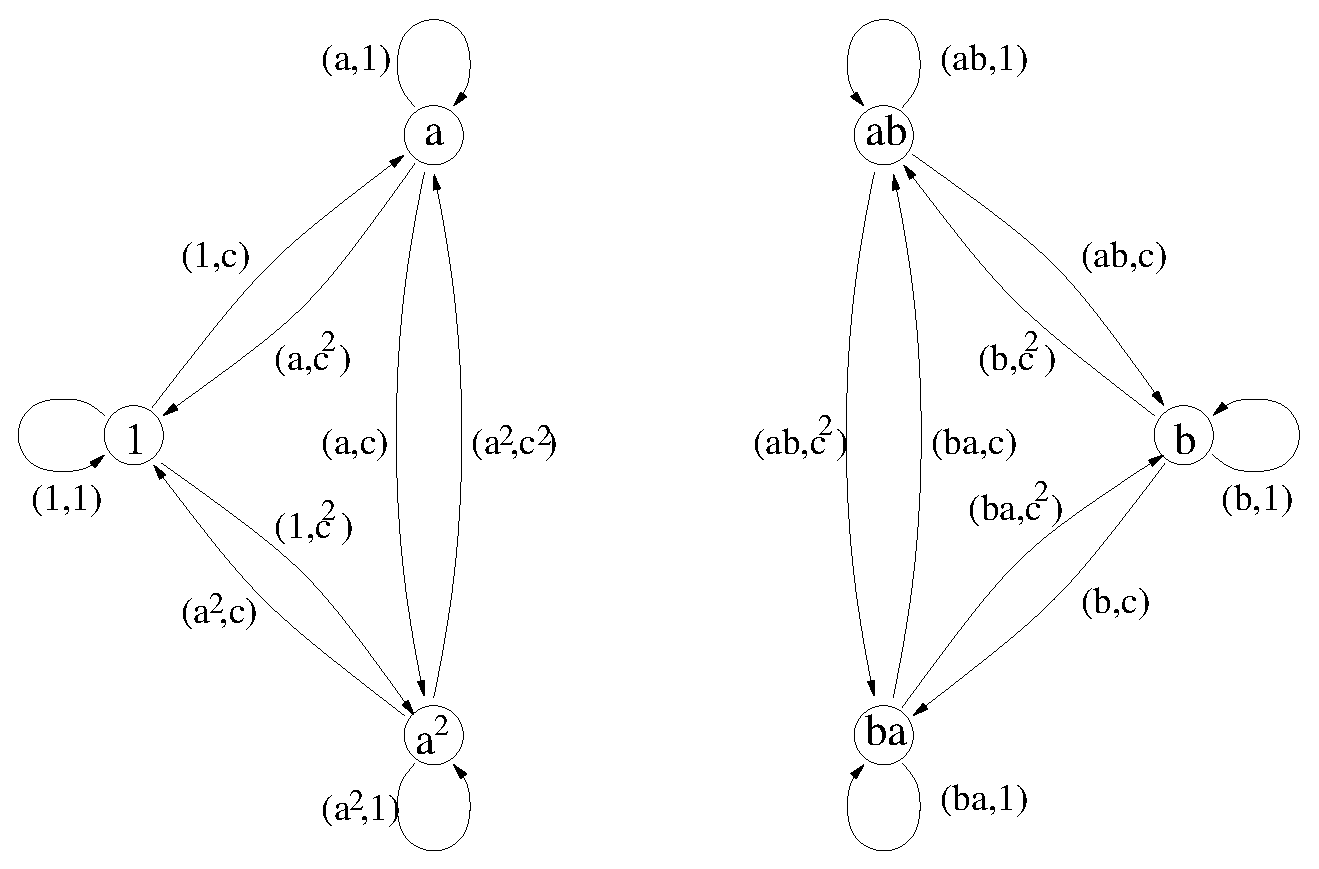
\includegraphics[scale = 0.60]{xmodcat1/s3ggpd.eps}
%% \input{s3ggpd.pstex_t} 
\end{center}

\noindent
\emph{We may compare the group multiplication with the groupoid multiplication
by calculating, for example,}
\begin{eqnarray*}
(a,c)(a^2,c) &=& (1,c^{a^2}c) ~=~ (1,c^2), \\
(a,c)*(a^2,c)     &=& (a,c)(a^2,1)^{-1}(a^2,c) ~=~ (a^4,c^{a^3}c) ~=~ (a,c^2).
\end{eqnarray*}
\end{example}

\begin{example} \label{ex:G18}
This example may be investigated in {\GAP} with the following corredpondence:
$$
a \mapsto (7,8,9),~ b \mapsto (8,9),~ c \mapsto (2,3)(4,5)
$$

{\small 
\begin{verbatim}
gap> G18 := GroupGroupoid( C18);
groupoid with 2 pieces:
1:  single piece groupoid with rays: < Group( [ ()>-()->() ] ), 
[ (), (7,8,9), (7,9,8) ], [ ()>-()->(), ()>-(4,6,5)->(7,9,8), 
  ()>-(4,5,6)->(7,8,9) ] >
2:  single piece groupoid with rays: < Group( [ (8,9)>-(2,3)(5,6)->(8,9) ] ), 
[ (8,9), (7,8), (7,9) ], [ (8,9)>-(2,3)(5,6)->(8,9), (8,9)>-(2,3)(4,5)->(7,8),
  (8,9)>-(2,3)(4,6)->(7,9) ] >
gap> piece2 := Pieces( G18 )[2];;
gap> obs2 := piece2!.objects;
[ (8,9), (7,8), (7,9) ]
gap> RaysOfGroupoid( piece2 );
[ (8,9)>-(2,3)(5,6)->(8,9), (8,9)>-(2,3)(4,5)->(7,8), 
  (8,9)>-(2,3)(4,6)->(7,9) ]
gap> elts2 := ElementsOfGroupoid( piece2 );;
gap> x := elts2[3];
[(8,9)>-(2,3)(4,6)->(7,9) : (8,9) -> (7,9)]
gap> y := elts2[8];
[(7,9)>-(1,3)(4,6)->(7,8) : (7,9) -> (7,8)]
gap> x*y;
[(8,9)>-(2,3)(4,5)->(7,8) : (8,9) -> (7,8)]
\end{verbatim}} 
\end{example} 


\newpage
%%%%%%%%%%%%%%%%%%%%%%%%%%%%%%%%%%%%%%%%%%%%%%%
\subsection{Regular Groupoids} \label{subs:reggpd} \index{regular groupoid} 

Let $\calX = (\partial : S \to R)$ be a precrossed module and let 
$\calC = (e;t,h : G \to R)$ be the associated precat$^1$-group 
where $G = R \ltimes S$ 
has multiplication $(r_1,s_1)(r_2,s_2) = (r_1r_2,s_1^{r_2}s_2)$ 
and inverse $(r,s)^{-1} = (r^{-1},(s^{-1})^{r^{-1}})$. 
The homomorphisms $e,t,h$ are given by 
$er = (r,1),~ t(r,s) = r,~ h(r,s) = r(\partial s)$. 

The associated group-groupoid $\calG$ has vertex set $R$ and arrows $G$ 
with the tail (source) and head (target) maps given by $t$ and $h$. 
Composition $*$ in $\calG$ is given by 
$$
(r_1,s_1) * (r_2,s_2) = (r_1,s_1)(r_2^{-1},1)(r_2,s_2) = (r_1,s_1s_2) 
$$ 
and is defined when $r_1(\partial s_1) = r_2$. 
The identity element in the object group at $r$ is $er = (r,1)$. 

\begin{defn} \label{defn:left-right-action}
Let $\calG$ be a groupoid with objects $R$ and arrows $G$. 
\begin{enumerate}[(i)]
\item
Maps $\rhd : R \times G \to G$ and $\lhd : G \times R \to G$ 
are respectively \emph{left} and \emph{right actions} of $R$ on $G$ 
if for all $q,r \in R$ and $g,h \in G$ 
\begin{itemize} 
\item 
$(qr) \rhd g = q \rhd (r \rhd g)$,~ $g \lhd (qr) = (g \lhd q) \lhd r$; 
\item
$q \rhd (g \lhd r) = (q \rhd g) \lhd r$; 
\item
$1 \rhd g = g = g \lhd 1$; 
\item
$t(r \rhd g) = r(tg)$,~ $t(g \lhd r) = (tg)r$,~ 
$h(r \rhd g) = r(hg)$,~ $h(g \lhd r) = (hg)r$; 
\item 
$r \rhd (g * g') = (r \rhd g) * (r \rhd g')$,~ 
$(g * g') \lhd r = (g \lhd r) * (g' \lhd r)$, 
whenever $g * g'$ is defined; 
\item 
$q \rhd er = e(qr) = eq \lhd r$. 
\end{itemize}
\item 
$\calG$ is \emph{semiregular} if $R$ is a monoid 
and if $\calG$ has left and right actions as in (i). 
\item
A semiregular $\calG$ is \emph{regular} if $R$ is a group. 
\end{enumerate}
\end{defn}

\begin{lem}
When $\calG$ is the group groupoid associated to a precat$^1$-group $\calC$, 
left and right actions are given by left and right multiplication:
$$
r \lhd g := (er)g, \qquad  g \rhd r := g(er).
$$
\end{lem}
\begin{pf}
We only verify the axioms for $\lhd$ since those for $\rhd$ follow similarly. 
\begin{eqnarray*}
g \lhd (qr) &=& g \lhd (eq)(er) = (g \lhd q)(er) = (g \lhd q) \lhd r; \\ 
q \rhd (g \lhd r) &=& q \rhd (g(er)) = (eq)g(er) 
                   =  ((eq)g) \lhd r = (q \rhd g) \lhd r; \\
g \lhd 1 &=& g(e1) = g; \\
t(g \lhd r) &=& t(g(er)) = (tg)(ter) = (tg)r; \\
h(g \lhd r) &=& h(g(er)) = (hg)(her) = (hg)r; \\
(g \lhd r)*(g' \lhd r) &=& (g(er))(eh(g(er)))^{-1}g'(er) 
     = g(er)(er)^{-1}(ehg)^{-1}g'(er) = (g*g') \lhd r; \\
eq \lhd r &=& (eq)(er) = e(qr). 
\end{eqnarray*}
\end{pf}

\begin{prop} 
Let $\calG$ be a semiregular groupoid. 
Then there are two everywhere defined binary operations on $G$ given by: 
\begin{eqnarray*}
g \circledcirc g' &=& (g \lhd tg') * (hg \rhd g'), \\ 
g \circledast g' &=& (tg \rhd g') * (g \lhd hg'). 
\end{eqnarray*} 
When $\calG$ is a regular groupoid both $\circledcirc$ and $\circledast$ 
make $G$ into a group with identity $e1$. 
\end{prop} 

Following on from the example above, when $\calG$ is a group groupoid, 
we find that $\circledcirc$ is just the multiplication in $G$. 
\begin{eqnarray*}
g \circledcirc g' &=& (g \lhd tg') * (hg \rhd g') \\
              &=& (g(etg'))*((ehg)g') \\ 
              &=& g(etg')(eh(g(etg')))^{-1}(ehg)g' \\ 
              &=& g(etg')((ehg)(etg'))^{-1}(ehg)g' \\ 
              &=& gg'. 
\end{eqnarray*} 
\noindent
The situation with $\circledast$ is a little more complicated: 
\begin{eqnarray*}
g \circledast g' &=& (tg \rhd g') * (g \lhd hg') \\ 
                 &=& ((etg)g')(eh((etg)g'))^{-1}(g(ehg') \\ 
                 &=& (etg)g')((etg)(ehg'))^{-1}g(ehg') \\ 
                 &=& (etg)g'(ehg')^{-1}(etg)^{-1}g(ehg'). 
\end{eqnarray*} 
Now $g'(ehg')^{-1} \in \ker h$ and $(etg)^{-1}g \in \ker t$. 
When $\calG$ is a cat$^1$-group these two products commute, 
so the expression reduces to $gg'$ and $\circledast$ is also 
just multiplication in $G$.


\newpage
%%%%%%%%%%%%%%%%%%%%%%%%%%%%%%%%%%%%%%%%%%%
\subsection{$2$-groups} \label{subs:twogps}

Finally, we think of such a structure as a special case of a 
\index{$2$-category} \index{$2$-group} \index{$2$-cell} 
$2$-category, which has objects, morphisms, and $2$-\emph{cells}.
We follow the presentation in Subsection 1.2.3 of 
Forrester-Barker's thesis \cite{f-b-thesis}. 
For an introduction to $2$-groupoids, 
see Kamps and Porter \cite{kamps:port}.
(Note that a $2$-group is \emph{not} a special case of the group theorist's 
$p$-group, with $p=2$, but is a $2$-category with one object having all 
morphisms and $2$-cells invertible.)

The $2$-group $\calH$ associated to $\calX = (\partial : S \to R)$ has
\begin{itemize}
\item  a single object $\bullet$,
\item  morphisms $r \in R$,
\item  $2$-cells $(r,s) \in R \ltimes S$
       with tail $r$ and head $r(\partial s)$.
\end{itemize}
$$
\xy
\xymatrix{
   & & & \\
 \Downarrow (r,s)~= 
   & \bullet  \ar@/^5ex/[rr]^{r} 
              \ar@/_5ex/[rr]_{r(\partial s)} 
     & \Downarrow (r,s)
        & \bullet \\
   & & & \\
}
\endxy
$$

%\medskip
\noindent
Horizontal composition $(r_1,s_1) \sharpz (r_2,s_2)$ 
of $2$-cells is given by
$$
\xy
\xymatrix{
  & &  & & & & & & \\
  \bullet \ar@/^5ex/[rr]^{r_1} 
          \ar@/_5ex/[rr]_{r_1(\partial s_1)} 
  & \Downarrow (r_1,s_1)
    & \bullet \ar@/^5ex/[rr]^{r_2} 
              \ar@/_5ex/[rr]_{r_2(\partial s_2)} 
      & \Downarrow (r_2,s_2)
        & \bullet 
          & = 
            & \bullet \ar@/^5ex/[rr]^{r_1r_2} 
                      \ar@/_5ex/[rr]_{r_1(\partial s_1)r_2(\partial s_2)} 
              & \Downarrow (r_1r_2,{s_1}^{r_2}{s_2})
                & \bullet \\
  & & & & & & & & \\
}
\endxy
$$

%\medskip
\noindent
There is a unique \emph{horizontal identity} $2$-cell
$$
\xy
\xymatrix{
   & & & \\
 \Downarrow(1,1)~=
   & \bullet  \ar@/^5ex/[rr]^{1} 
             \ar@/_5ex/[rr]_{1} 
     & \Downarrow (1,1)
        & \bullet \\
   & & & \\
}
\endxy
$$

%\medskip
\noindent
Similarly, when $r_1(\partial s_1) = r_3$,
vertical composition $(r_1,s_1) \sharpo (r_3,s_3)$ 
of $2$-cells is given by
$$
\xy
\xymatrix{
  && && & & && \\
  && \Downarrow (r_1,s_1)
     && & & && \\
  \bullet \ar@/^15ex/[rrrr]^{r_1} 
          \ar[rrrr]^{r_1(\partial s_1)}
          \ar@/_15ex/[rrrr]_{r_1(\partial s_1)(\partial s_3)} 
  && && \bullet 
        &=& \bullet \ar@/^5ex/[rr]^{r_1} 
                    \ar@/_5ex/[rr]_{r_1(\partial(s_1s_3))} 
            & \Downarrow (r_1,s_1s_3)
             & \bullet \\
  && \Downarrow (r_1(\partial s_1),s_3)
     && & & && \\
  && && & & && \\
}
\endxy
$$

\medskip\noindent
For each $r \in R$ there is a \emph{vertical identity} $2$-cell 
$$
\xy
\xymatrix{
   & & & \\
 \Downarrow(r,1)~=
   & \bullet  \ar@/^5ex/[rr]^{r} 
             \ar@/_5ex/[rr]_{r} 
     & \Downarrow (r,1)
        & \bullet \\
   & & & \\
}
\endxy
$$
such that
$$
\Downarrow(r,1)\; \sharpo \Downarrow(r,s)\; 
                  \sharpo \Downarrow(r(\partial s),1)
~=~ \Downarrow(r,s).
$$

The \emph{horizontal inverse} and the 
\emph{vertical right inverse} of ~$\Downarrow(r,s)$~ 
are ~$\Downarrow(r^{-1},(s^{-1})^{r^{-1}})$~ and \\  
$\Downarrow(r(\partial s),s^{-1})$~ respectively.

Horizontal composition with vertical identities is called 
\emph{whiskering}. 
In diagrams it is often convenient to shrink ~$\Downarrow(q,1)$~ 
to a single arc, labelled $q$, as in the whiskering formlae:
$$
q_1 \sharpz \Downarrow(r,s) ~\sharpz~ q_2 
~=~ \Downarrow(q_1rq_2,{s}^{q_2}).
$$

\bigskip\noindent
The Peiffer condition for cat$^1$-groups establishes an 
\index{Peiffer condition} \index{interchange law} 
\emph{interchange law} for $\calH$,
$$
((r_1,s_1) \sharpz (r_2,s_2)) \sharpo ((r_3,s_3) \sharpz (r_4,s_4))
\quad = \quad
((r_1,s_1) \sharpo (r_3,s_3)) \sharpz ((r_2,s_2) \sharpo (r_4,s_4)) 
$$
for the well-defined composite 
when $r_1(\partial s_1) = r_3$ and $r_2(\partial s_2) = r_4$,
$$
\xy
\xymatrix{
  && && && && \\
  && \Downarrow (r_1,s_1)
     && && \Downarrow (r_2,s_2)
           && \\
  \bullet \ar@/^15ex/[rrrr]^{r_1} 
          \ar[rrrr]^{r_1(\partial s_1) = r_3}
          \ar@/_15ex/[rrrr]_{r_3(\partial s_3)} 
  && && \bullet \ar@/^15ex/[rrrr]^{r_2} 
                \ar[rrrr]^{r_2(\partial s_2) = r_4}
                \ar@/_15ex/[rrrr]_{r_4(\partial s_4)} 
        && && \bullet \\
  && \Downarrow (r_3,s_3)
     && && \Downarrow (r_4,s_4)
           && \\
  && && && && \\
}
\endxy
$$

\noindent
When this composite is defined, 
$$
    s_2{s_3}^{r_4}
~=~ s_2{s_3}^{r_2(\partial s_2)}
~=~ {s_3}^{r_2}s_2
$$
and the composite $2$-cell is
$$
\xy
\xymatrix{
   && && \\
   \bullet \ar@/^5ex/[rrrr]^{r_1r_2} 
           \ar@/_5ex/[rrrr]_{r_3(\partial s_3)r_4(\partial s_4)} 
   && \Downarrow (r_1r_2,(s_1s_3)^{r_2}s_2s_4)
      && \bullet \\
   && && \\
}
\endxy
$$

